%Pakete;
%A4, Report, 12pt
\documentclass[ngerman,a4paper,12pt]{scrreprt}
\usepackage[a4paper, right=20mm, left=20mm,top=30mm, bottom=30mm, marginparsep=5mm, marginparwidth=5mm, headheight=7mm, headsep=15mm,footskip=15mm]{geometry}

%Papierausrichtungen
\usepackage{pdflscape}
\usepackage{lscape}

%Deutsche Umlaute, Schriftart, Deutsche Bezeichnungen
\usepackage[utf8]{inputenc}
\usepackage[T1]{fontenc}
\usepackage[ngerman]{babel}

%quellcode
\usepackage{listings}
\usepackage{verbatim}

%tabellen
\usepackage{tabularx}
\usepackage{csvsimple}

%listen und aufzählungen
\usepackage{paralist}

%farben
\usepackage[svgnames,table,hyperref]{xcolor}

%font
\usepackage{helvet}
\renewcommand{\familydefault}{\sfdefault}

%Abkürzungsverzeichnisse
\usepackage[printonlyused]{acronym}

%Bilder
\usepackage{graphicx} % Bilder
\usepackage{float}	  %"Floating" Objects, Bilder, Tabellen...

%Pdf einbinden
\usepackage{pdfpages}


%Dokumenteigenschaften
\title{Dkoumentation Simulationsprojekt Hardrock}
\def\author{Reto Schelbert, Simon Schreiber, Tobias Blaser, Urs Baumann}
\providecommand{\teacher}{A. Rinkel}
\providecommand{\room}{5.002}
\providecommand{\versionnumber}{2.0}
\date{\today{}, Rapperswil}


%Kopf- /Fusszeile
\usepackage{fancyhdr}
\usepackage{lastpage}

\pagestyle{fancy}
\fancyhf{} %alle Kopf- und Fußzeilenfelder bereinigen
\fancyhead[L]{System Modelling and Simulation} %Kopfzeile links
\fancyhead[C]{Projekt: Hardrock} %Kopfzeile mitte
\fancyhead[R]{Seite \thepage/\pageref{LastPage}} %Kopfzeile rechts
\renewcommand{\headrulewidth}{0.4pt} %obere Trennlinie
\fancyfoot[L]{\jobname} %Fusszeile links
\fancyfoot[C]{Version: \versionnumber} %Fusszeile mitte
\fancyfoot[R]{\today{}} %Fusszeile rechts
\renewcommand{\footrulewidth}{0.4pt} %untere Trennlinie

%Kopf-/ Fusszeile auf chapter page
\fancypagestyle{plain} {
	\fancyhf{} %alle Kopf- und Fußzeilenfelder bereinigen
	\fancyhead[L]{System Modelling and Simulation} %Kopfzeile links
	\fancyhead[C]{Projekt: Hardrock} %Kopfzeile mitte
	\fancyhead[R]{Seite \thepage/\pageref{LastPage}} %Kopfzeile rechts
	\renewcommand{\headrulewidth}{0.4pt} %obere Trennlinie
	\fancyfoot[L]{\jobname} %Fusszeile links
	\fancyfoot[C]{Version: \versionnumber} %Fusszeile mitte
	\fancyfoot[R]{\today{}} %Fusszeile rechts
	\renewcommand{\footrulewidth}{0.4pt} %untere Trennlinie
}

\usepackage{changepage}

%links, verlinktes Inhaltsverzeichnis, PDF Inhaltsverzeichnis
\usepackage[bookmarks=true,
bookmarksopen=true,
bookmarksnumbered=true,
breaklinks=true,
colorlinks=true,
linkcolor=black,
anchorcolor=black,
citecolor=black,
filecolor=black,
menucolor=black,
pagecolor=black,
urlcolor=black
]{hyperref} % Paket muss unbedingt als letzes eingebunden werden!

\begin{document}

%Titel und Inhaltsverzeichnis
\thispagestyle{empty}
\begin{titlepage}
	\begin{center}

	\vspace*{40mm}
	
	\begin{figure}[htp]
		\centering
		
\includegraphics[width=0.60\textwidth]{img/Hard-Rock-Cafe-Logo-Black-White.png}
	\end{figure}		
	\vspace*{20mm}
	
	{\fontsize{40}{48} \selectfont Projekt Hardrock \\[10mm]}
	{\fontsize{32}{48} \selectfont Dokumentation \\[5mm]}	
	\vspace*{20mm}
	\author

\end{center}
\end{titlepage}
\clearpage

\chapter*{Änderungsnachweis}
\begin{tabularx}{\textwidth}{|cXlr|} % Versionstabelle, Rahmen links und rechts
		\hline
		\textbf{Version} & \textbf{Änderung} & \textbf{Autor} & \textbf{Datum}\\
		\hline
		1.0 & Dokumentenentwurf & Tobias Blaser & 24.03.2013 \\
		1.1 & Entwurf Konzept & Tobias Blaser & 28.03.2013 \\
		1.2 & Ergänzungen und Korrekturen & Reto Schelbert & 03.04.2013 \\
		1.3 & Überarbeitung Konzept (Word Model) & Tobias Blaser & 08.04.2013 \\
		1.4 & Modell \& Verteilungsfunktionen & Tobias Blaser & 03.05.2013 \\
		1.5 & Simulation & Alle & 10.05.2013 \\
		1.6 & Modellbeschreibungen & Tobias Blaser & 11.05.2013\\
		1.7 & Plausibilitätscheck, Szenarios & Alle & 13.05.2013\\
		1.8 & Szenarien, Auswertung & Urs Baumann, Tobias Blaser & 17.05.2013\\
		1.9 & Auswertung, Überarbeitungen & Alle & 24.05.2013\\
		2.0 & Überarbeitungen & Alle & 27.05.2013\\
		\hline
\end{tabularx}

% Inhaltsverzeichnis
\tableofcontents


\chapter{Konzept}


\section{Model}
Als Ausgangskonzept wird das Hardrock in Atlantic City verwendet.
\begin{figure}[htp]
	\centering
		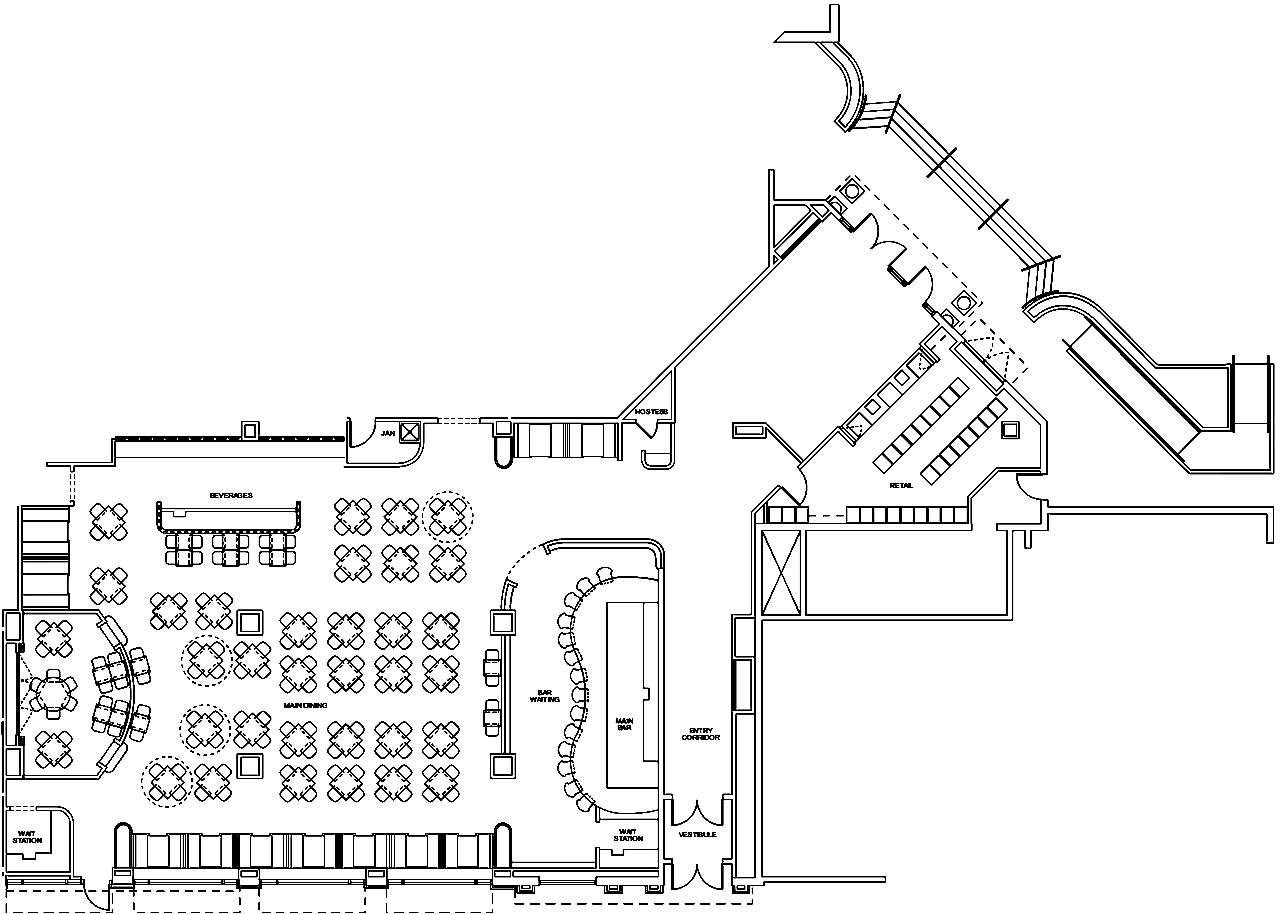
\includegraphics[width=1\textwidth]{img/hardrock-plan.png}
		\caption[Gebäudeplan Hardrock]{Gebäudeplan Hardrock Cafe, Atlantic City (Quelle: www.hardrock.com, 25.03.13)}
		\label{planHardrock}
\end{figure}

\subsection{Eingangsbereich}
Vor dem Eingangsbereich warten die Gäste in einer Schlange, bis an der Bar Plätze frei werden. Ziel ist, diese Warteschlange so kurz wie möglich zu halten. 

Ist die Schlange vor dem Eingang zu lang, verlassen die Gäste das Restaurant wieder ohne Konsumation. Dies soll möglichst vermieden werden, da diese Gäste keinen Umsatz bescheren. Sind dagegen Plätze an der Bar frei, so bewegen sich die Gäste direkt dort hin.

\subsection{Bar}
Die Bar dient als Warteschlange für die Gäste, bis Plätze an einem Tisch frei werden. Gäste werden an der Bar mit Getränken bedient.

In der Realität wäre das Ziel, dass die Bar optimal besetzt ist, weil dies zusätzliche Einnahmen durch Konsumation generiert. Gleichzeitig sollte vor der Türe die Schlange möglichst klein sein oder gar nicht existieren, damit keine Gäste an der Kälte warten müssen, oder sogar wieder gehen. Die Wartezeit an der Bar sollte nicht mehr als ein bis zwei Drinks betragen, damit niemand wieder geht, bevor ein Tisch frei wird.

Das Barpersonal soll in unserer Simulation nicht berücksichtigt werden. Grund dafür ist die Unabhängigkeit des Barbereichs vom Rest des Lokals. Das heisst: Das Barpersonal ist nicht in der Lage, kurzzeitig die Bar zu verlassen und Tische zu bedienen. Weil das Barpersonal nur für die Ausgabe der Getränke verantwortlich ist, kann es in der Simulation vernachlässigt werden, ohne das System zu verfälschen. Zudem gehen wir von einer fixen Bargrösse aus und beziehen auch den durch die Bar erzielten Umsatz nicht in die Simulation mit ein.

\subsection{Tische}
Am Tisch werden ein bis drei Gänge gegessen. In einem ersten Schritt soll dies sehr einfach abgebildet werden. Auf eine komplexe Menüsimulation in der Granularität der einzelnen Gänge wird verzichtet.

Das Servicepersonal bewegt sich ein einziges Mal zum Tisch und nimmt Bestelllungen auf. Das Servicepersonal ist somit pro Tisch ein Mal für eine bestimmte Zeit belegt und anschliessend wieder frei.

Ein Szenario, in dem das Servicepersonal mehrfach an einem Tisch vorbeikommt -- z.B. um das Gedeck, Teller und Karte zu bringen und den Tisch am Ende wieder abzuräumen -- soll erst in einem zweiten Schritt modelliert werden, je nach verfügbarer Projektzeit.

In der realen Welt bestehen die Tische aus Vierertischen. Ankommende Gruppen müssen entweder aufgeteilt oder Tische zusammengeschoben werden, damit Gruppen zusammen sitzen können. Bei Gruppen von weniger als 4 Personen kann es unbesetzten Plätzen an den Tischen kommen: Ein einzelner Gast setzt sich selten zu einer Gruppe von 3 Personen an einem Vierertisch. Um die Simulation nicht unnötig aufzublähen, soll dies nicht berücksichtigt werden.
Die Anzahl Plätze werden fix gewählt anhand des Beispiels von Atlantic City (250 Plätze).

Nach dem Esssen  verlassen die Gäste das Hardrock Cafe und der Tisch wird frei für neue Gäste.
In der Realität kann es durchaus vorkommen, dass Gäste nach dem Essen nochmals an die Bar zurückkehren. Auch dies soll in der Simulation nicht berücksichtigt werden.


\subsection{Küche}
	In der Küche werden die verschiedenen Mahlzeiten gekocht und angerichtet. Die Köche arbeiten gleichzeitig an mehreren Menüs und versuchen, alle zu einer Gruppe von Gästen gehörenden Mahlzeiten  gleichzeitig fertigzustellen.

	In einem ersten Schritt soll die Küche sehr rudimentär simuliert werden. Es existieren Köche, die eine bestimmte Zeit benötigen, um Essen zuzubereiten. Paralleles Kochen von Mahlzeiten soll nur durch entsprechende Verkürzung der Gesammtkochzeit abgebildet werden.

	In einem zweiten Schritt könnnten verschiedene Köche, die pro Mahlzeit und Gang für eine bestimmte Zeit gebunden sind, modelliert werden.


\section{Bewegungsabläufe}
	\begin{figure}[H]
		\centering
			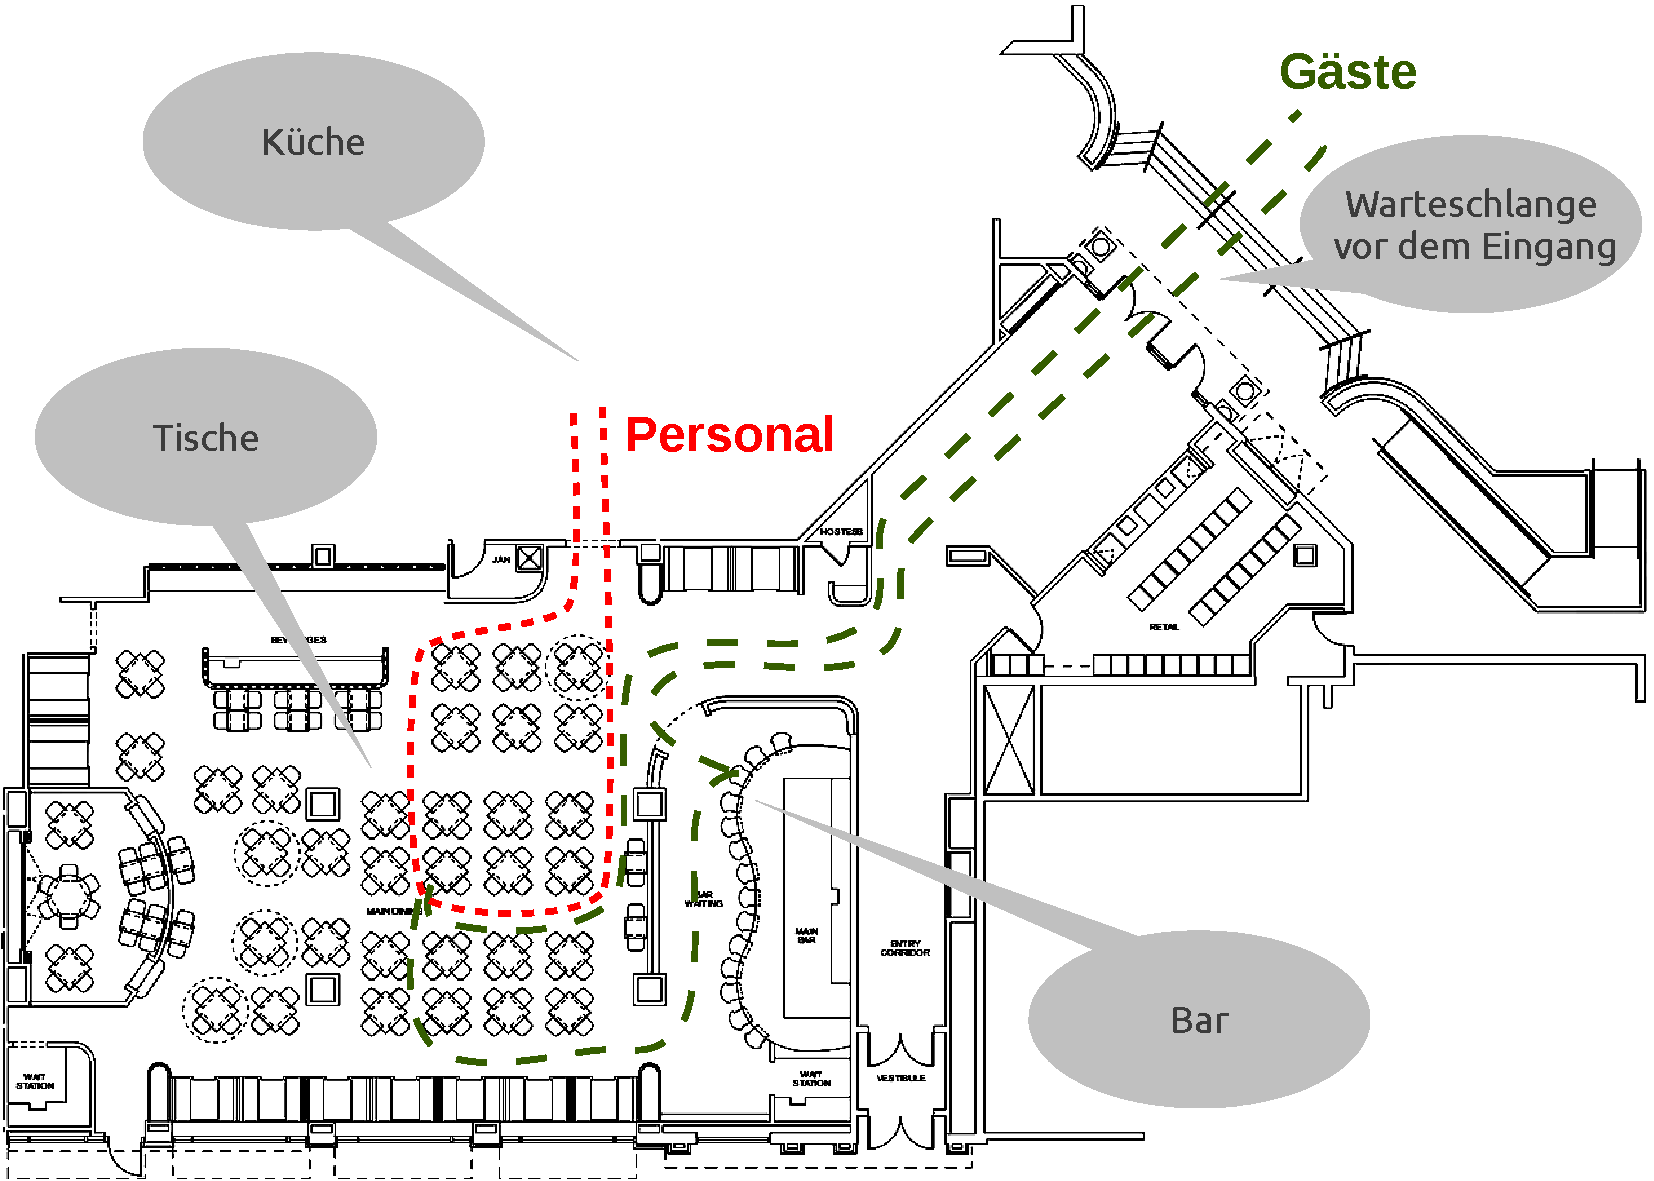
\includegraphics[width=1\textwidth]{img/hardrockSchema.pdf}
			\caption[Bewegungsschema Hardrock]{Bewegungsschema im Hardrock Cafe, Atlantic City (Beispiel Bewegungsablauf an einem Tisch)}
			\label{schemaHardrock}
	\end{figure}

	Die verschiedenen Aktivitäten finden an unterschiedlichen Orten im Café statt. Die daraus resultierenden Wegzeiten variieren stark, unterliegen sehr komplexen Verteilungen und können nur empirisch ermittelt werden.

	\subsection{Gäste}
		\begin{itemize}
			\item Gäste benötigen eine variierende Zeit um vom Eingang an die Bar zu gelangen. 
			\item Gäste benötigen eine variierende Zeit, um von der Bar zum zugewiesenen Tisch zu gelangen.
			Diese kann von der Gruppengrösse, der Anordnung der Tische und der Belegung des Restaurants (verschiedene "Gästeströme") abhängen. Diesen Umstand berücksichtigen wir in der Simulation jedoch nur durch eine Variation der Wegzeit -- unabhängig von den beeinflussenden Faktoren.
			\item Gäste benötigen eine variierende Zeit, um das Lokal wieder zu verlassen.
		\end{itemize}

	\subsection{Personal}
		\begin{itemize}
			\item Köche bewegen sich nur innerhalb der Küche
			\item Das Servicepersonal benötigt eine variierende Zeit einerseits für den Weg von Tisch zu Tisch und andrerseits für den Weg von der Küche zu den Tischen.
			\item Die Tellerbinger benötigen je nach Tisch unterschiedlich viel Zeit, um von der Küche zu den Tischen zu gelangen.
			\item Servicepersonal, Tellerbringer und Gäste beeinflussen sich gegenseitig in den Wegzeiten: Eine grosse Anzahl von Personen im Raum führt zu Verzögerungen bei allen Laufwegen. Theoretisch kann es auch zu Zusammenstössen kommen. Dies wird in der Simulation nicht berücksichtigt.
		\end{itemize}

	\subsection{Realität und Simulation}
		Für die Simulation sollen sinnvolle Annahmen über das Verhalten der Wegzeiten getroffen werden und die gegenseitige Beeinflussung der Gäste und des Personals gegenseitig und untereinander vernachlässigt werden. Eine zusätzliche 2D/3D Animation wäre sehr aufwändig, was den Rahmen dieses Projektes sprengen würde.



\section{Warum soll simuliert werden?}
	\begin{itemize}
		\item Das Szenario ist zu komplex, um alle einfliessenden Faktoren in statischen Berechnungen zu berücksichtigen. Es sind zu  viele Variablen im Spiel.
		\item Gegenseitige Beeinflussung der Faktoren: Das System Restaurant eignet sich für die Simulation, da die Werte wie Umsatz und Auslastung von verschiedenen Faktoren abhängen und eine einfache Berechnung deshalb nicht möglich ist. Die Wahl und Anzahl der Ressourcen wie Anzahl Köche, Servicepersonal und Tellerbringer ist entscheidend für das Funktionieren des Systems. Zudem beeinflussen sich die Ressourcen gegenseitig und stehen in Abhängigkeit zueinander.
		\item Gebäudebau: Aus Kostengründen ist es nicht möglich einen Prototypen zu bauen und darin zu testen.
		\item Ist das Gebäude einmal gebaut, so sind  architektonische Veränderungen, die sich aus einer falschen Annahme der Anzahl von Gästen und Mitarbeitern ergeben (Anzahl Kochplätze, Grösse der Bar, Abstand der Tische zueinander) nur mit grossem Kostenaufwand realisiert werden.
		\item Testen durch Reallife-Simulation ist nicht möglich, weil Statisten beim Warten sterben würden, vom vielen Essen dick würden oder verhungern würden beim Warten auf die Bestellung. Möglicherweise würden Sie auch an der Bar zu viele Drinks nehmen und wären zu betrunken um an einen Tisch zu wechseln.
		\item Zudem tauchen Unsicherheiten auf durch Verteilungen,  Streuungen und Variabilitäten in der Anzahl der Gäste, Serviceagents und deren Servicetime, Warteschlangen und Wartezeiten.
	\end{itemize}

\section{Objectives}
	\subsection{Gewinn}
	Ziel ist die Gewinnmaximierung durch gute Belegung des Restaurants. Zu optimieren ist die Anzahl des Personals im Hinblick auf dieses Ziel. Die Anzahl des Personals im Service, in der Küche und im Tellerbringen ist voneinander abhängig. Hautpziel ist, die optimale Anzahl für den jeweiligen Bereich zu bestimmen. 

	\subsection{Utilization}
	Indirekt abhängig von der Utiliziation der beteiligten Ressourcen ist das Ziel der Gewinnmaximierung. So ist zum Beispiel ein nicht ausreichend ausgelastetes Servicepersonal mit Kosten verbunden, denen keine Einnahmen in Form von verkauften Mahlzeiten gegenüber steht.
	  
	\subsection{Dauer des Aufenthalts}
		Ebenfalls ein Hinweis auf geringen Umsatz ist eine zu kurze mittlere Aufenthaltszeit am Tisch oder sehr lange Wartezeiten der Gäste auf bestellte Mahlzeiten. Wir gehen davon aus, dass die Aufenthaltsdauer bei ca. 1.5 Stunden liegt und die mittlere Wartezeit für die Bedienung 15 Minuten nicht übersteigt.

\section{Spezifikationen}
	Gearbeitet wird mit fiktiven Daten, ausgenommen die Anzahl der Plätze im Saal. Diese werden vom Hardrock Atlantic City übernommen.

	\subsection{Variable Grössen}
		Es sollen verschiedene Szenarien simuliert werden. Die dazu benötigten Grössen sollen Variabel sein:
		\begin{itemize}
			\item Queuelänge
			\item Anzahl Servicepersonal
			\item Anzahl Tellerbringer
			\item Anzahl Köche
			\item Gruppen mit unterschiedlichen Anzahlen von Gästen
		\end{itemize}

	\subsection{Resultatgrössen}
		Durch die Simulation sollen die Aufenthaltszeiten ermittelt werden, z.B. die \textbf{Dauer des Aufenthaltes und Wartezeiten am Tisch}, die \textbf{Gesamtaufenthaltsdauer im Restaurant} und die \textbf{Auslastung der Agents}.
Zusätzlich soll anhand von festgelegten Kosten der Gewinn berechnet werden.

\subsection{Zusatzprojekt (optional)}
	In einem weiteren Projekt kann die Simulation ausgebaut und verfeinert werden, indem weitere Parameter hinzugefügt  und detailliertere Daten erhoben werden:
	\begin{itemize}
		\item Anzahl Personal an der Bar
		\item Verschiedene Essen/Menüs mit unterschiedlichen Servicezeiten für die Köche.
		\item Gruppen müssten zusammen an einem Tisch untergebracht werden, keine Leerplätze.
		\item Weitere Resultate: Wie lange dauert die Bestellaufnahme, wie lange muss ein Gast durchschnittlich auf die Bestellung warten und wie lange wartet er auf die Rechnung? Wie oft muss das Servicepersonal an einen Tisch gehen pro Gast?
		\item Optional: Kleine Animation
	\end{itemize}


\chapter{Modellierung}
	\section{Activities}
		\begin{figure}[H]
			\centering
				\includegraphics[page=4,trim=1cm 3cm 2.5cm 1cm, clip=true,width=\textwidth]{../model/Modell_v2.pdf}
				\caption[Activity Diagramm]{Activity Diagramm}
				\label{activityDiagramm}
		\end{figure}
		
		\subsection{Gastgruppe}
		Eine Gastgruppe belegt während dem Aufenthalt am Tisch Plätze. Anschliessend wird Servicepersonal benachrichtigt um eine Bestellung zu erstellen.
		Entsprechend den Anzahl Gängen werden soviele Gänge angeliefert.
		Vor den Verlassen des Lokals wird Bezahlt, anschliessend werden die Plätze wieder freigegeben.
		
		\subsection{Service}
		Das Servicepersonal befindet sich in einem geschlossenen Zyklus. Es nimmt am Tisch eine oder mehrere Bestellungen auf und bringt diese in die Küche.
		
		\subsection{Köche}
		Die Köche befinden sich ebenfalls in einem geschlossenen Zyklus. Sie nehmen Bestellungen entgegen und richten Teller an.
		
		\subsection{Tellerbringer}
		Auch die Tellerbringer befinden sich in einem geschlossenen Zyklus. Sie holen angerichtete Teller ab und bringen Sie an den Tisch.
		

\begin{landscape}
	\section{Hardrock Guest Flow}
		\begin{figure}[H]
			\centering
				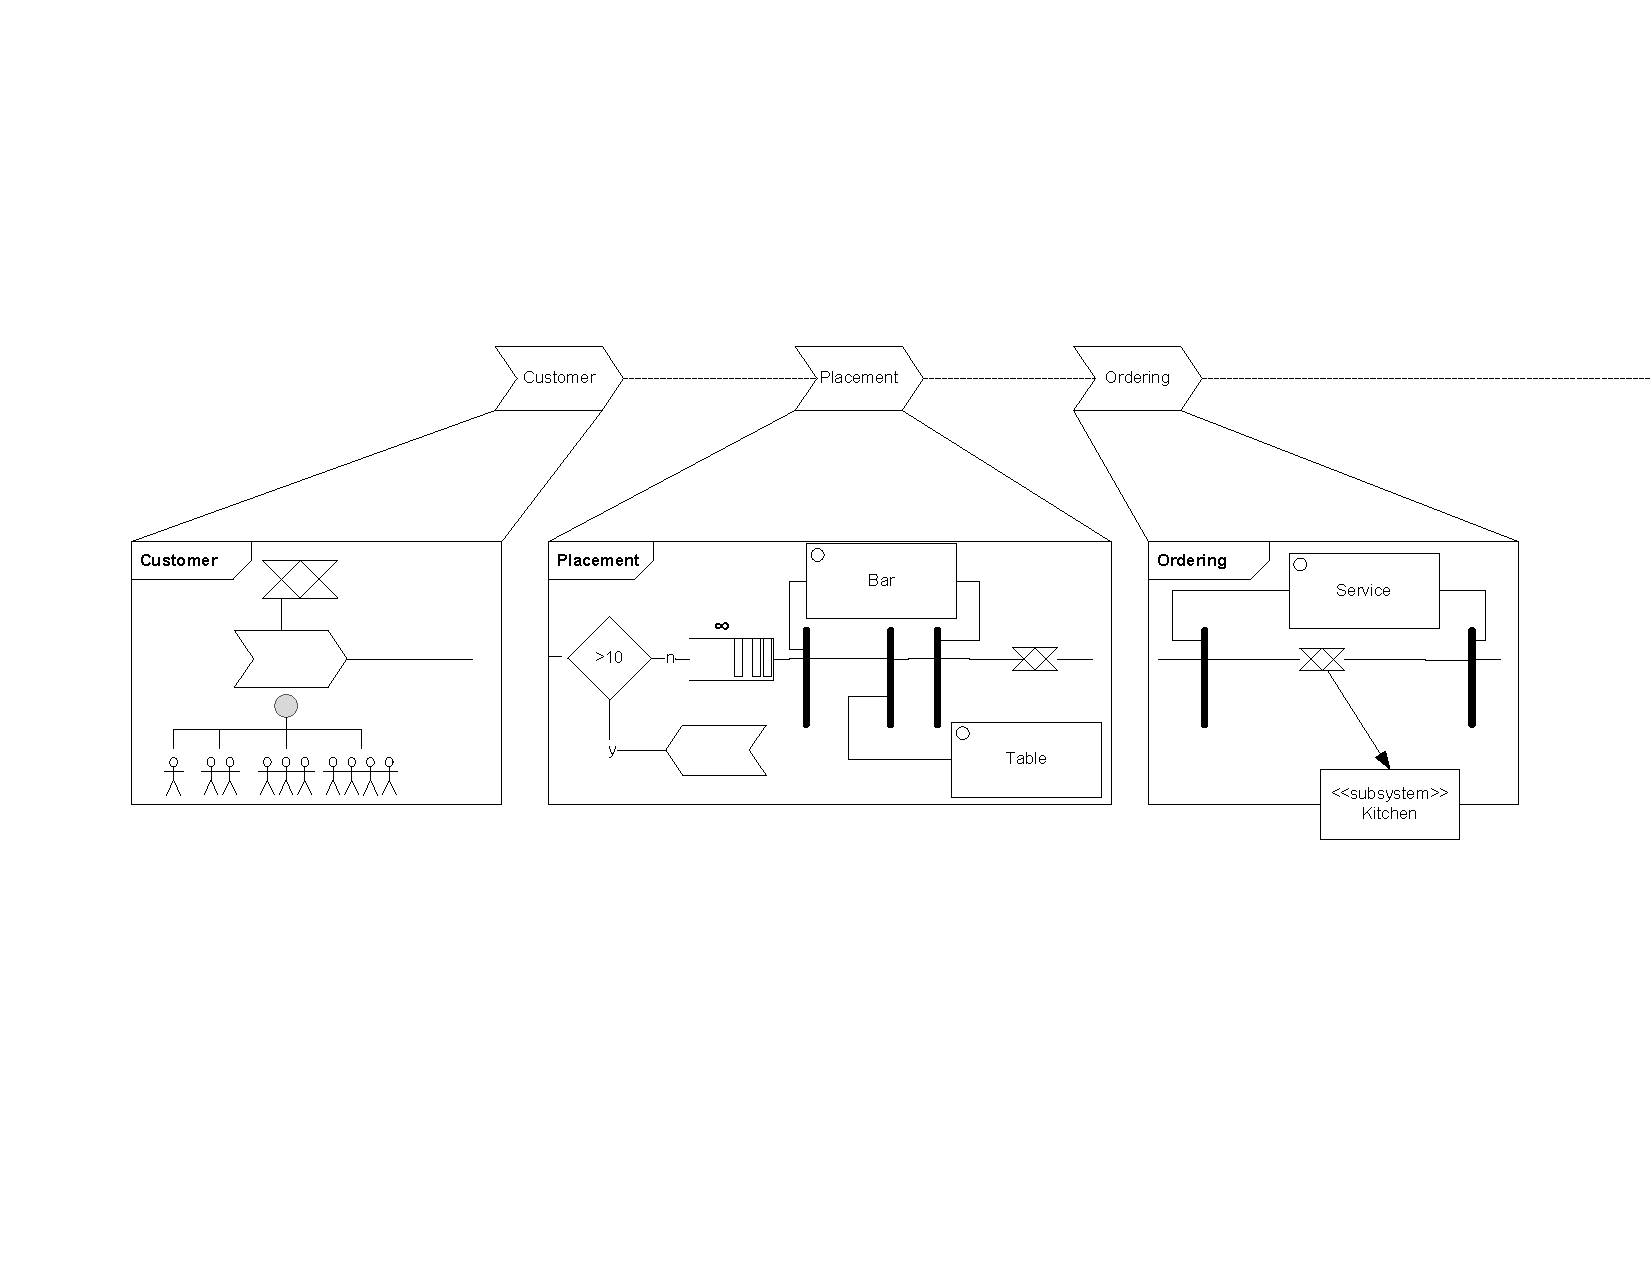
\includegraphics[page=1,trim=2cm 7cm 2cm 5cm, clip=true,width=1.4\textwidth]{../model/Modell_v2.pdf}
				\caption[Hardrock Flow Diagramm Teil1]{Hardrock Flow Diagramm Teil1}
				\label{flowDiagramm1}
		\end{figure}
		
		\subsection{Customer}
		Gäste werdem in Gruppen von eins bis vier Personen erzeugt. Die Erzeugung unterliegt einer definierten Verteilung.
		
		\subsection{Placement}
		Gäste warten in einer Queue, bis eine Platzressource zur Belegung an der Bar frei wird. Sollte diese Queue die Länge von 10 Gruppen übsteigen, was im Mittel ca. 20 Leuten entspricht, werden neu ankommende Gäste das Hardrock wieder verlassen. Die Anzahl verlorener Gäste wird am Schluss ermittel. Die Platzressource wird freigegeben, sobald eine freie Tischressource belegt werden kann.
		
		\subsection{Ordering}
		Während einer Bestellung wird die Bedienung als Ressource belegt und anschliessend wieder freigegeben.
		
		\begin{figure}[H]
				\includegraphics[page=2,trim=0cm 7cm 2cm 5cm, clip=true,width=1.4\textwidth]{../model/Modell_v2.pdf}
				\caption[Hardrock Flow Diagramm Teil2]{Hardrock Flow Diagramm Teil2}
				\label{flowDiagramm2}
		\end{figure}
		
		\subsection{Dinnering}
		Gäste warten, bis die Bestellung zubereitet wurde (Verteilfunktion). Für die Auslieferung der Teller wird die Ressource Tellerbringer für eine bestimmte Zeit (Verteilfunktion) belegt. Die Dauer des Essens wird ebenfalls mittels einer Verteilfunktion modelliert.
		
		Wenn Gäste mehrere Gänge bestellt haben, so kommen auch mehrmals die Tellerbringer und bringen das Gekochte.
		
		\subsection{Payment}
		Für die Bezahlung ist bis jetzt kein Szenario definiert, sie wird hier nur der Vollständigkeit Willen aufgeführt.
		
		\subsection{Exit}
		Gäste geben die belegte Ressource Tisch wieder frei und verlassen das Restaurant.
		
		\subsection{Kitchen}
		Die Bestellung der Gruppe wird in einzelneUnterbestellungen aufgesplittet (je nach Gruppengrösse 1-4) und kann parallel verarbeitet werden. Eine Unterbestellung belegt eine Ressource Koch für die Dauer der Zubereitung, welche mittels einer Verteilfunktion bestimmt wird.
		
		\begin{figure}[H]
			\begin{center}
					\includegraphics[page=3,trim=2cm 12cm 12cm 2cm, clip=true,width=0.6\textwidth]{../model/Modell_v2.pdf}
					\caption[Hardrock Flow Diagramm Kitchen]{Hardrock Flow Diagramm Kitchen}
					\label{flowDiagrammKitchen}
			\end{center}
		\end{figure}
		
		
\end{landscape}

		\subsection{Entitäten}
		Zusammengefasst sind in der Modellierung des Systems die folgenden Entitäten vorhanden.
		
		\begin{itemize}
			\item Vor der Türe:
				\begin{itemize}
					\item Queue: Ankommende Gäste
				\end{itemize}
			\item Küche
				\begin{itemize}
					\item Agents: Köche
				\end{itemize}
			\item Bedienung
				\begin{itemize}
					\item Agents: Servicepersonal, Tellerbringer
				\end{itemize}
			\item Bar
				\begin{itemize}
					\item Queue: Anzahl Warteplätze
				\end{itemize}
			\item Tische
				\begin{itemize}
					\item Ressourcen: Anzahl Plätze
				\end{itemize}
			\item Gäste
				\begin{itemize}
					\item Entities: Gruppen von 1-4 Personen 
				\end{itemize}
	\end{itemize}


\chapter{Simulation mit Arena}
	\section{Customer}			
		\subsection{Verteilung der ankommenden Gäste}
			Um die Verteilung des Andrangs, insbesondere die beiden Spitzenzeiten am Mittag und am Abend, zu simulieren, nutzen wir einen Schedule. Die Ankunftsrate im Scheduler wird durch eine negative Exponentialverteilung bestimmt.
	
			\begin{figure}[H]
				\centering
					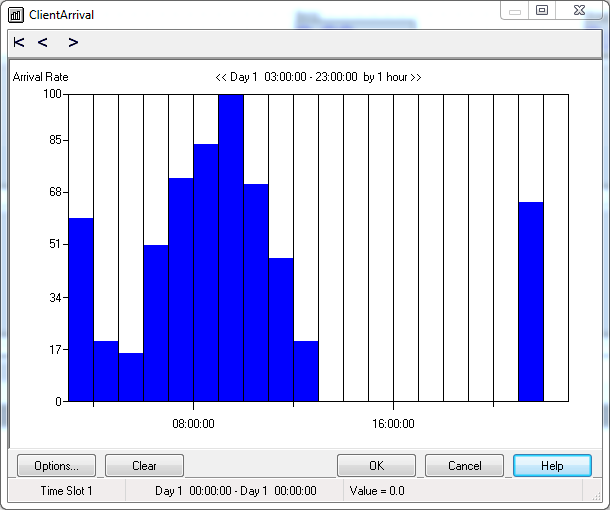
\includegraphics[trim=0.35cm 1.75cm 1cm 1.75cm, clip=true,width=0.75\textwidth]{img/scheduler.png}
					\caption[Arrival Sceduler in Arena]{Ankunfts Sceduler in Arena}
					\label{arrivalSceduler}
			\end{figure}
	
			\subsubsection{Gruppengrösse}
			Einer angekommenden Entität wird anschliessend eine zufällige Gruppengrösse zwischen eins und vier Personen zugeteilt. Dazu wird eine Triangularfunktion mit einem Mittelwert von 2 verwendet und der Ausgabewert auf die nächste ganze Zahl gerundet.
			
	
	\section{Placement}
		\begin{figure}[H]
			\centering
				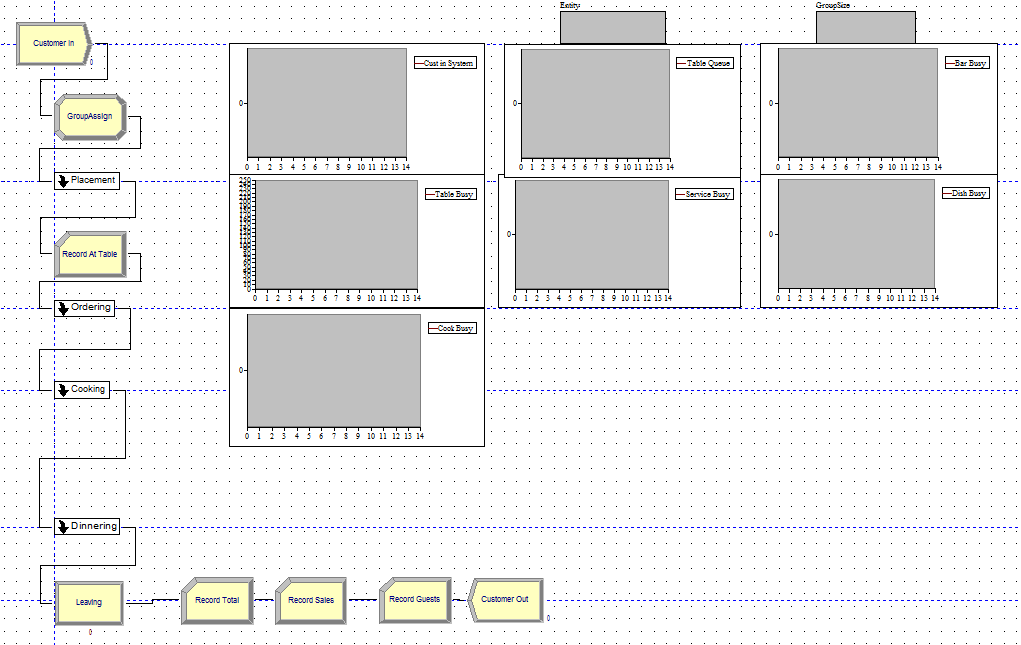
\includegraphics[width=\textwidth]{img/arena.png}
				\caption[Simulationsaufbau in Arena]{Aufbau einer ersten Simulation in Arena mit Submodels}
				\label{arenaSimulationsAufbau}
		\end{figure}
		
		\subsection{Überlauf am Eingang}
			Warten zu viele Gäste vor dem Eingang, werden weitere Gruppen abgeschreckt und kehren wieder um.
		
			Für die Simulation wird eine fixe Grösse verwendet: 			Befinden sich in der EntryQueue weniger als 10 Gruppen, so stellt sich die neue Gruppe an, andernfalls nicht. Mittels einem alternativen Dispose werden die abgeschreckten Gruppen gezählt.
			
			
		\subsection{Assignement und Release von Warteschlange, Bar und Tisch}
			In Arena wird das Assign/Release mittels Ressourcen umgesetzt. Als erstes wird die EntryQueue zugewiesen. Sobald an der Bar Plätze frei werden, wird die BarQueue assigned. Erst wenn der Platz an der BarQueue assigned ist, wird die EntryQueue released. Genau gleich wird für den Wechsel von der Bar an den Tisch verfahren.
	
	
		\subsection{Laufweg der Gäste von der Bar zum Tisch}
			Für den Weg von der Bar zum Tisch wird eine Uniformverteilung von eins bis fünf Minuten eingesetzt. Der Grund liegt darin, dass sich die Gruppen im Restaurant oft weit auseinander setzen. Es entstehen unterschiedliche Laufzeiten, da Tische näher oder weiter entfernt von der Bar platziert sind. Da die Entfernung der Tische keine Häufung aufweist und wir von einer gleichmässigen Auslastung aller Tische ausgehen, wird die Wegverteilung als uniform angenommen.
	
	
	\section{Ordering}			
		\subsection{Bestellvorgang}
			Das Erreichen des Tisches durch die Bedienung und die Bestellungsaufnahme werden zusammengefasst und mittels einer Triangularverteilung mit einem Mittelwert von 6 sowie einem Minimum von 3 und Maximum von 8 abgebildet. Pro Person am Tisch wird eine Minute aufgeschlagen, um die Abhängigkeit der Bestellzeit von der Gruppengrösse zu realisieren. Zudem ist in dieser grosszügigen Zeitberechnung der Anteil für einen zweiten Besuch am Tisch und die zusätzlichen Aufgaben wie Bereitmachen und Abräumen des Tisches enthalten.
	
	
	\section{Preparation}	
		\subsection{Verteilung der Zubereitungszeit}
			Für die Verteilung der Kochzeit wählen wir eine Normalverteilung mit einem Mittelwert von fünf und einer Standardabweichung von drei Minuten. Da im Hardrock verschiedenste Speisen zubereitet werden, von Salaten über Hauptgängen bis Desserts, ist die Normalverteilung hier die sinnvollste Abbildung. Die Kochzeit wird so kurz gewählt, weil ein guter Koch durch kochen von mehreren Menüs gleichzeitig Synergien nutzen kann.
	
	
		\subsection{Gruppenbestellungen}
			Gruppen bestellen gemeinsam und erhalten ihr Essen zum gleichen Zeitpunkt, gekocht wird es jedoch unabhängig. Um dies abzubilden, verwenden wir folgendes Vorgehen: Die Bestellung der Gruppe wird in der Küche in einzelne Bestellungen unterteilt und damit werden bis zu vier Unterbestellungen simuliert. Vor dem Ausliefern werden die Unterbestellungen wieder zu einer Gesamtbestellung zusammengefügt.
			
			
	\section{Dinnering}
		\subsection{Bestellungsauslieferung}					
			Die Tellerbringer liefern immer nur Gesamtbestellungen an eine Gruppe aus. Darum wird Bestellung nur ein Tellerbringer benötigt, der bis zu vier Teller (maximale Gruppengrösse) zum Tisch bringt. Zur Simulation wird die Laufzeit von der Theke bis zum Tisch in einer Uniformverteilung von einer halben bis vier Minuten abgebildet.


		\subsection{Essen}
			Das Essen dauert zwischen 15 Minuten und einer Stunde. Einzelne Gänge des Essens werden nicht konkret unterschieden, sondern nur implizit über die Dauer des Aufenthalts am Tisch in einer Verteilfunktion simuliert. Genutzt wird eine Triangularverteilung mit einem Mittelwert von 40 Minuten.\\
			
		\begin{figure}[H]
			\centering
				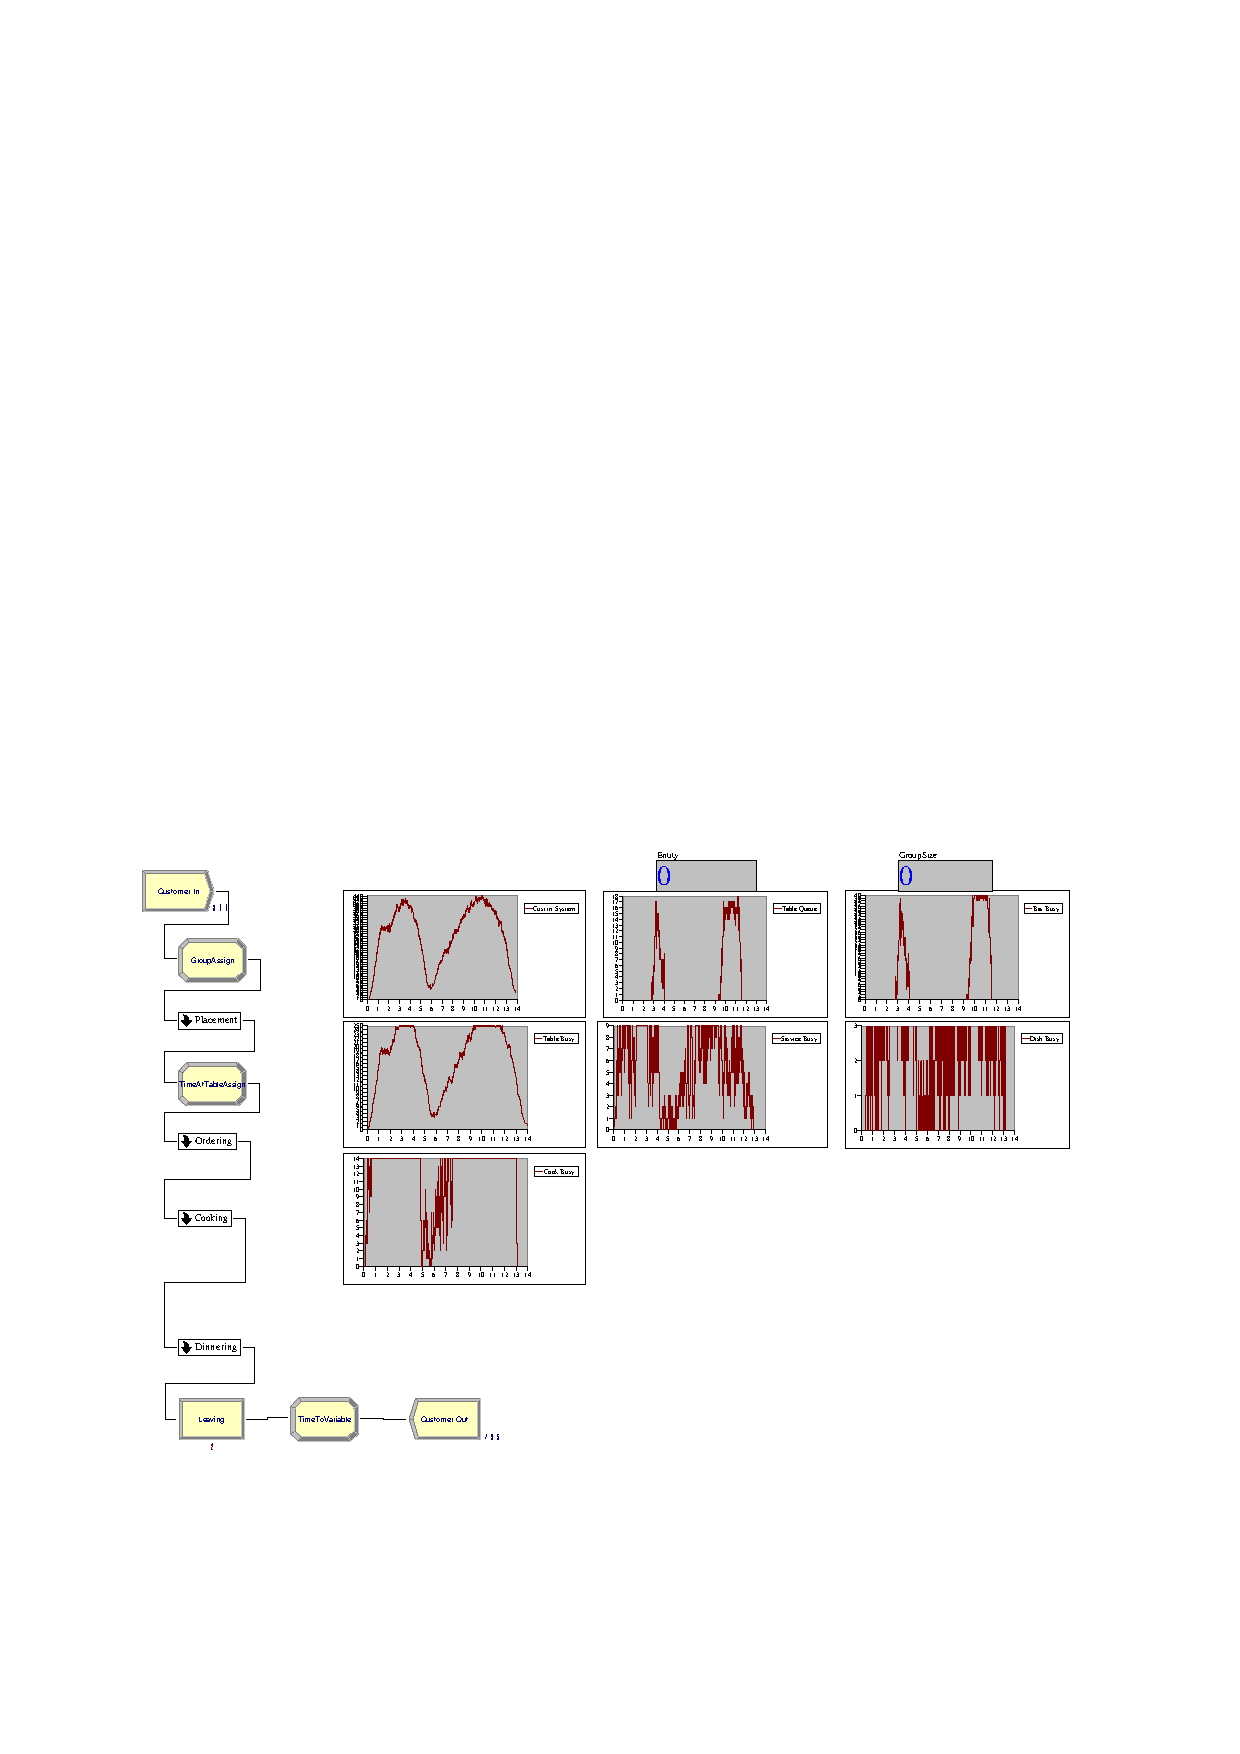
\includegraphics[trim=5.5cm 7.5cm 2.5cm 15cm, clip=true,width=\textwidth]{img/Model11a.pdf}
				\caption[Diagramme in Arena]{Überwachung der Simulation in Arena mit Diagrammen}
				\label{arenaDiagramme}
		\end{figure}	
			
			
	\section{Szenarien}
		Zur einfacheren Realisierung der Szenarien wird in Arena das Tool Process Analyzer genutzt. Damit können Szenarien definiert werden, die die Simulation mit den definierten Parametern beliebig viele Male aufrufen und die Resultate wieder zusammenführen. \\
		
		Die Szenarien sollen in einem ersten Schritt aufzeigen, in welcher Grössenordnung sich die Anzahl der benötigten Servicekräfte, Tellerbringer und Köche zueinander bewegt. In weiteren Schritten sollen die Szenarien ähnlich einer Lawinensuche auf den jeweils besten Bereich eingeschränkt und verfeinert werden.
			
			
	\section{Plausibilitäts-Checks}
	Zur Überprüfung der Plausibilität des aufgebauten Arena Modells experimentierten wir mit verschiedenen Parametern. Dabei sind einige Dinge aufgefallen:
	\begin{itemize}
		\item Die minimale Grösse der Bar muss der grösst möglichen Gruppengrösse (in unserem Fall 4) entsprechen. Andererseits können Gruppen, die grösser als die Bar sind, gar nicht ins Restaurant eintreten.
		Dieses Szenario entspricht nicht ganz der Realität. In der Realität bestehen grosse Gruppen aus kleineren Gruppen. Daher wird ein Teil einer grossen Gruppe bereits das Restaurant betreten, während die Restlichen noch draussen warten.\\
		$\rightarrow$ Da wir eine Bar zwischen 10 und 50 Plätzen anstreben und die Gruppen eine maximale Grösse von vier Personen ausweisen, spielt diese Gegebenheit keine Rolle.
		\item Fünf Angestellte im Service und drei Tellerbringer sind trotz 250 Gästen zu wenig ausgelastet. Das scheint für die Realität wenig plausibel.\\
		$\rightarrow$ Als Korrektur werden Lauf- und Bestellzeiten für das Servicepersonal und die Tellerbringer angepasst.
		\item Den Flaschenhals in der Simulation stellen die Köche dar. Die tiefe Utilization des Servicepersonals ergibt sich daraus, dass die Zubereitung der Essen zu lange dauert. Um dieses Verzerrung zu beheben, muss die Anzahl der Köche im Verhältnis zur Anzahl Servicepersonal erhöht werden.
		
		Gleichzeitig bringt das Servicepersonal in der Realität noch Getränke, Speisekarte, Gedecke, weist dem Gast den Tisch, räumt ab und steht für Fragen zur Verfügung.
		$\rightarrow$ Wir verzichten in unserer Simulation darauf, dies abzubilden. Da die Zeit für die Bedienung aber grosszügig berechnet ist, können die zusätzlichen Zeiten als darin enthalten betrachtet werden.
		\item Die benutzten Zeitvariablen zur Erfassung von Zeitstempeln im System basieren auf TNOW, wobei TNOW scheinbar kein Stempel zurückgibt, mit dem gerechnet werden kann.\\
		$\rightarrow$ TNOW muss zuerst in Basetime konvertiert werden. Wobei noch beachtet werden muss, dass die Basetime vom Run Setup abhängig ist.
	\end{itemize}
			
	\section{Umsatz}
\noindent
	Um den generierten Umsatz zu berechnen, setzen wir die folgenden Werte ein:
Die Kosten für Angestellte sind konstant und nicht von der Anzahl Bestellungen / Besucher abhängig. Deshalb wird wird der Lohn den Ressourcen als Kosten fix zugeteilt.\\

\begin{tabularx}{\textwidth}{|l|l|X|}
		\hline
		\textbf{Bezeichnung} & \textbf{Preis CHF} & \textbf{Verteilung}  \\
		\hline
		Menu & 20-60 & TRIA(20,30,60)  \\
		\hline
		Stundenlohn Koch & 25 & konstant (Mittelwert)\\
		Stundenlohn Tellerbringer & 20 & konstant (Mittelwert) \\
		Stundenlohn Servicepersonal & 25 & konstant (Mittelwert)\\
		\hline
\end{tabularx}
	
\chapter{Auswertung}
	\section{Szenarien}
			Gestartet wird mit 24 Szenarien, die sich verdoppelden Anzahlen von Angestellten in jedem Bereich (2, 4, 8, 16, 32) und Variationen beinhalten.
		
		\begin{figure}[H]
			\centering
				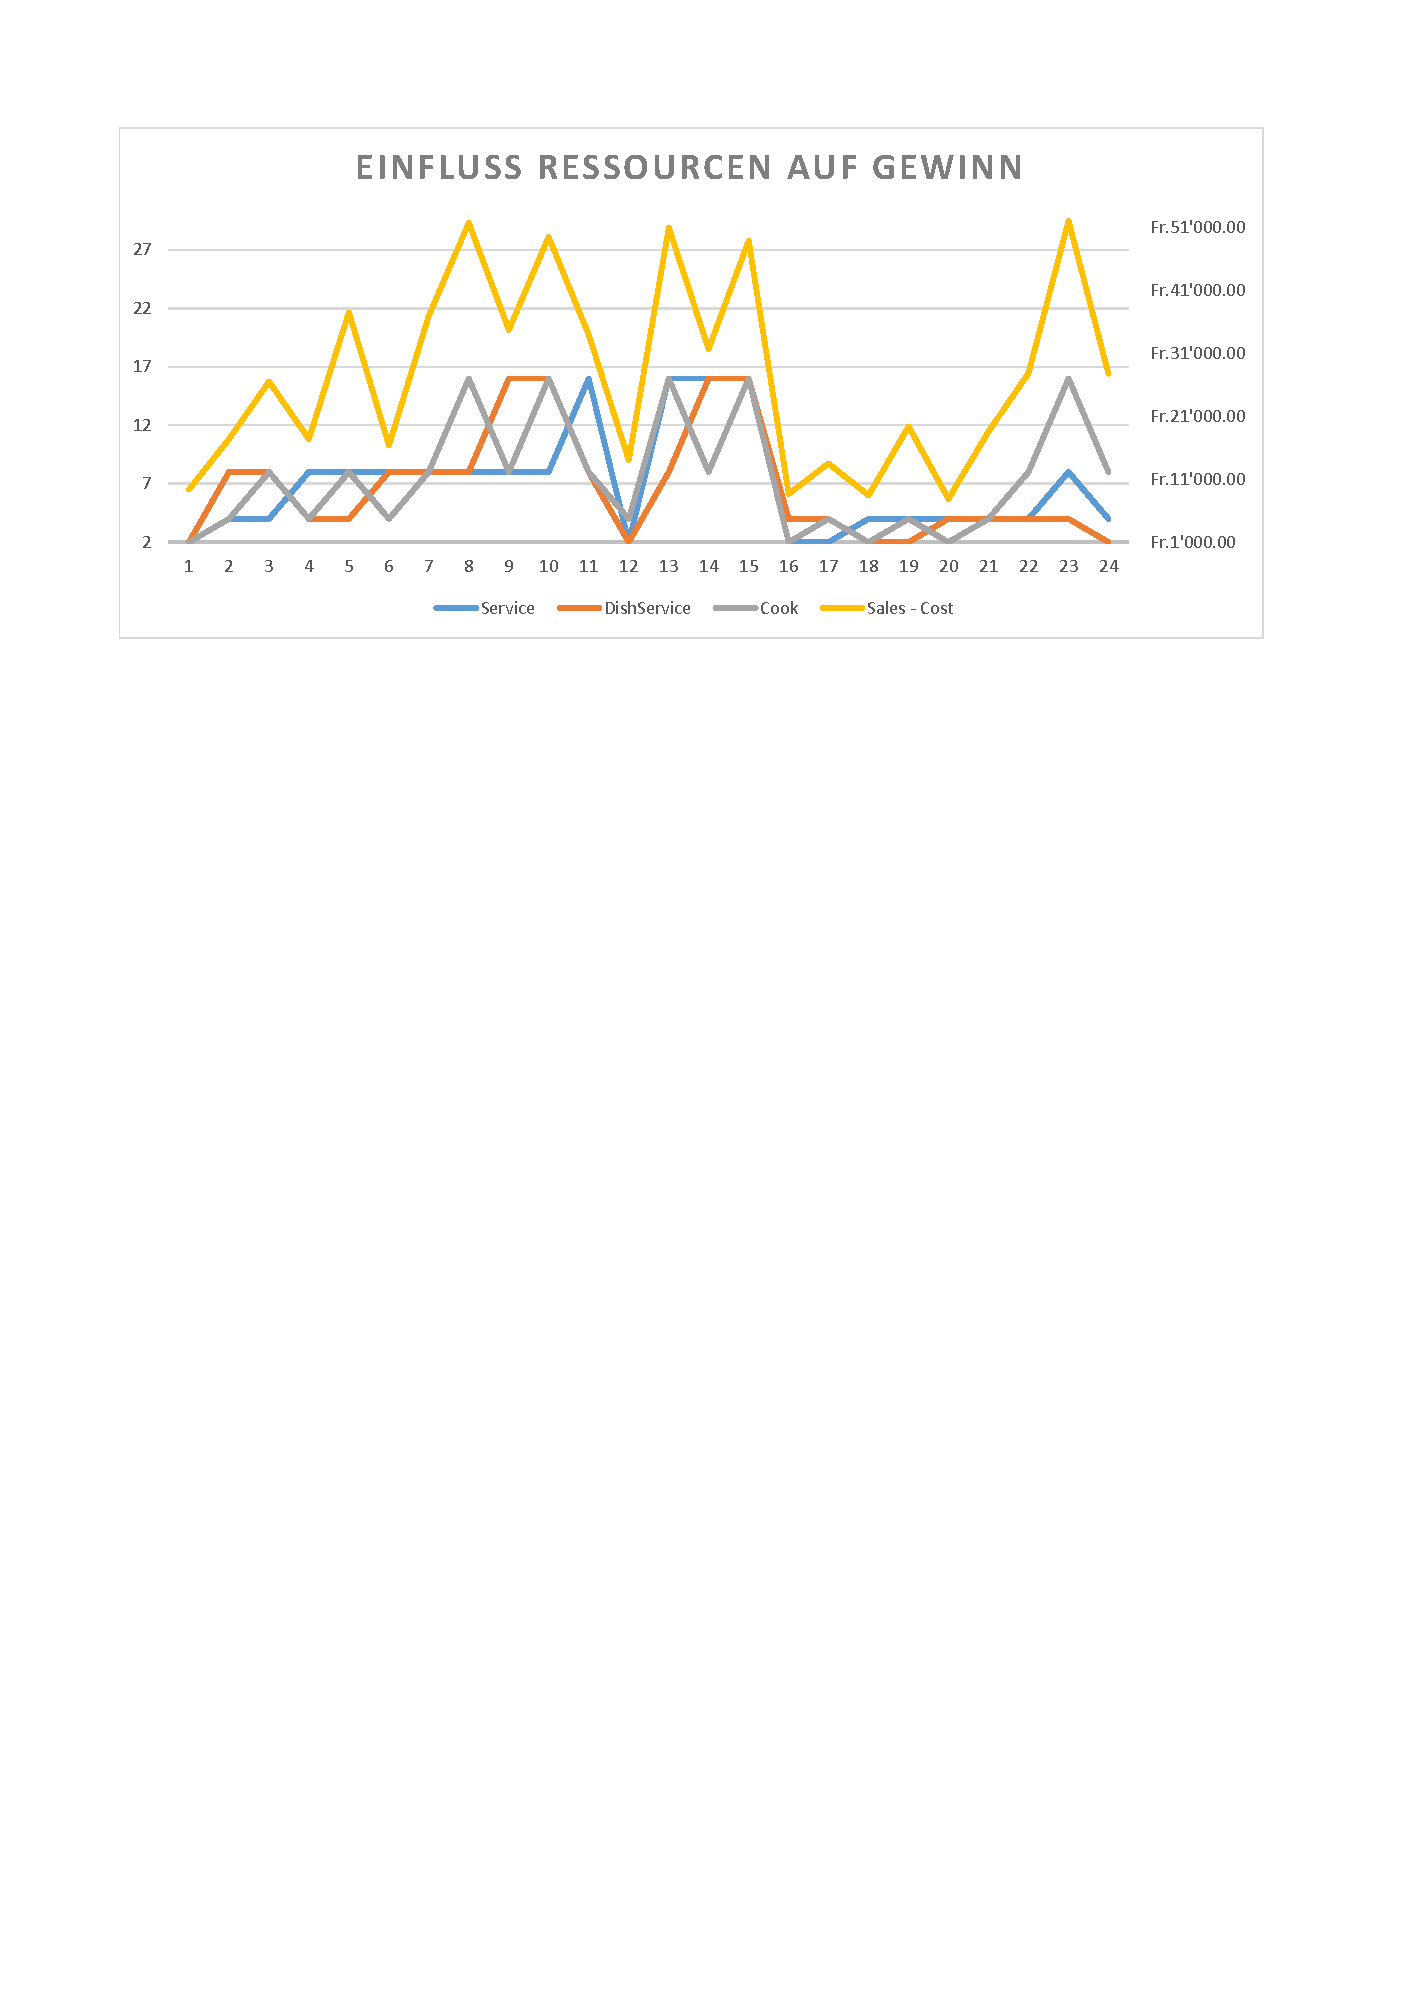
\includegraphics[trim=2cm 22.75cm 2cm 2cm, clip=true,width=\textwidth]{../Auswertung/1_groberOptimumBereich.pdf}
				\caption[Grobszenarien]{Grobszenarien (Y\textsubscript{left}: Mitarbeiter / X: Szenario / Y\textsubscript{right}: Gewinn)}
				\label{grobszenarien}
		\end{figure}
		
			
		\subsection{Szenarienoptimierung}
		Nach einer ersten Simulation hat sich herausgestellt, dass einige der oben definierten Szenarien gleich von Anfang an ausgeschlossen werden können. So zeigte sich, dass die Anzahl der Tellerbringer und Servicekräfte nicht über der Anzahl Köche liegen kann. Dies wurde ersichtlich, weil sich der Umsatz und damit der Durchsatz (Servicezeiten) im System nicht änderte wenn die Anzahl der Tellerbringer und Servicekräfte variiert wurde und diese überhalb der Anzahl Köche lag. Lediglich deren Utilization verringerte sich bei einer Erhöhung der Anzahl.
		 
		\subsection{erste Selektion}
			Bezogen auf die Umsatzoptimierung lassen sich aus den besten vier und den schlechtesten vier Szenarien die folgenden Tendenzen ableiten:
			\begin{itemize}
				\item Es werden viele Köche benötigt. 
				\item Tellerbringer braucht es sehr wenige.
				\item Beim Servicepersonal werden etwa halb so viele wie Köche und doppelt so viele wie Tellerbringer benötigt.
			\end{itemize}
		
			Aus diesen Daten entnehmen wir anschliessend den besten Fall (8 Servicepersonal, 4 Tellerbringer und 16 Köche) und analysieren diesen detaillierter:
		
			\begin{itemize}
				\item Der Service ist mit fast 90\% zu hoch ausgelastet. Konkret ist das Personal nicht nur zu den im Scheduler definierten Spitzenzeiten komplett ausgelastet, sondern über den ganzen Zeitraum mit Ausnahme in den Nachmittagsstunden. 				
				\item Die Tellerbringer sind zwar über die ganze Simulationszeit regelmässig ausgelastet, insgesamt jedoch zu wenig.
				\item Die Köche sind sehr konstant über die gesamte Simulationszeit ausgelastet.
			\end{itemize}
			
			
		\subsection{zweite Selektion}
			Als erstes erhöhen wir die Anzahl Simulationsdurchgänge von 10 auf 100, um stabilere und vertrauenswürdigere Resultate zu erhalten.
			
			\subsubsection{Servicepersonal}
				In einer erneuten Simulation wird nur die Anzahl Servicepersonal zwischen 8 und 14 variiert, während die Anzahl Tellerbringer bei 4 und die Anzahl Köche bei 16 bleibt.
				
				\begin{figure}[H]
					\centering
						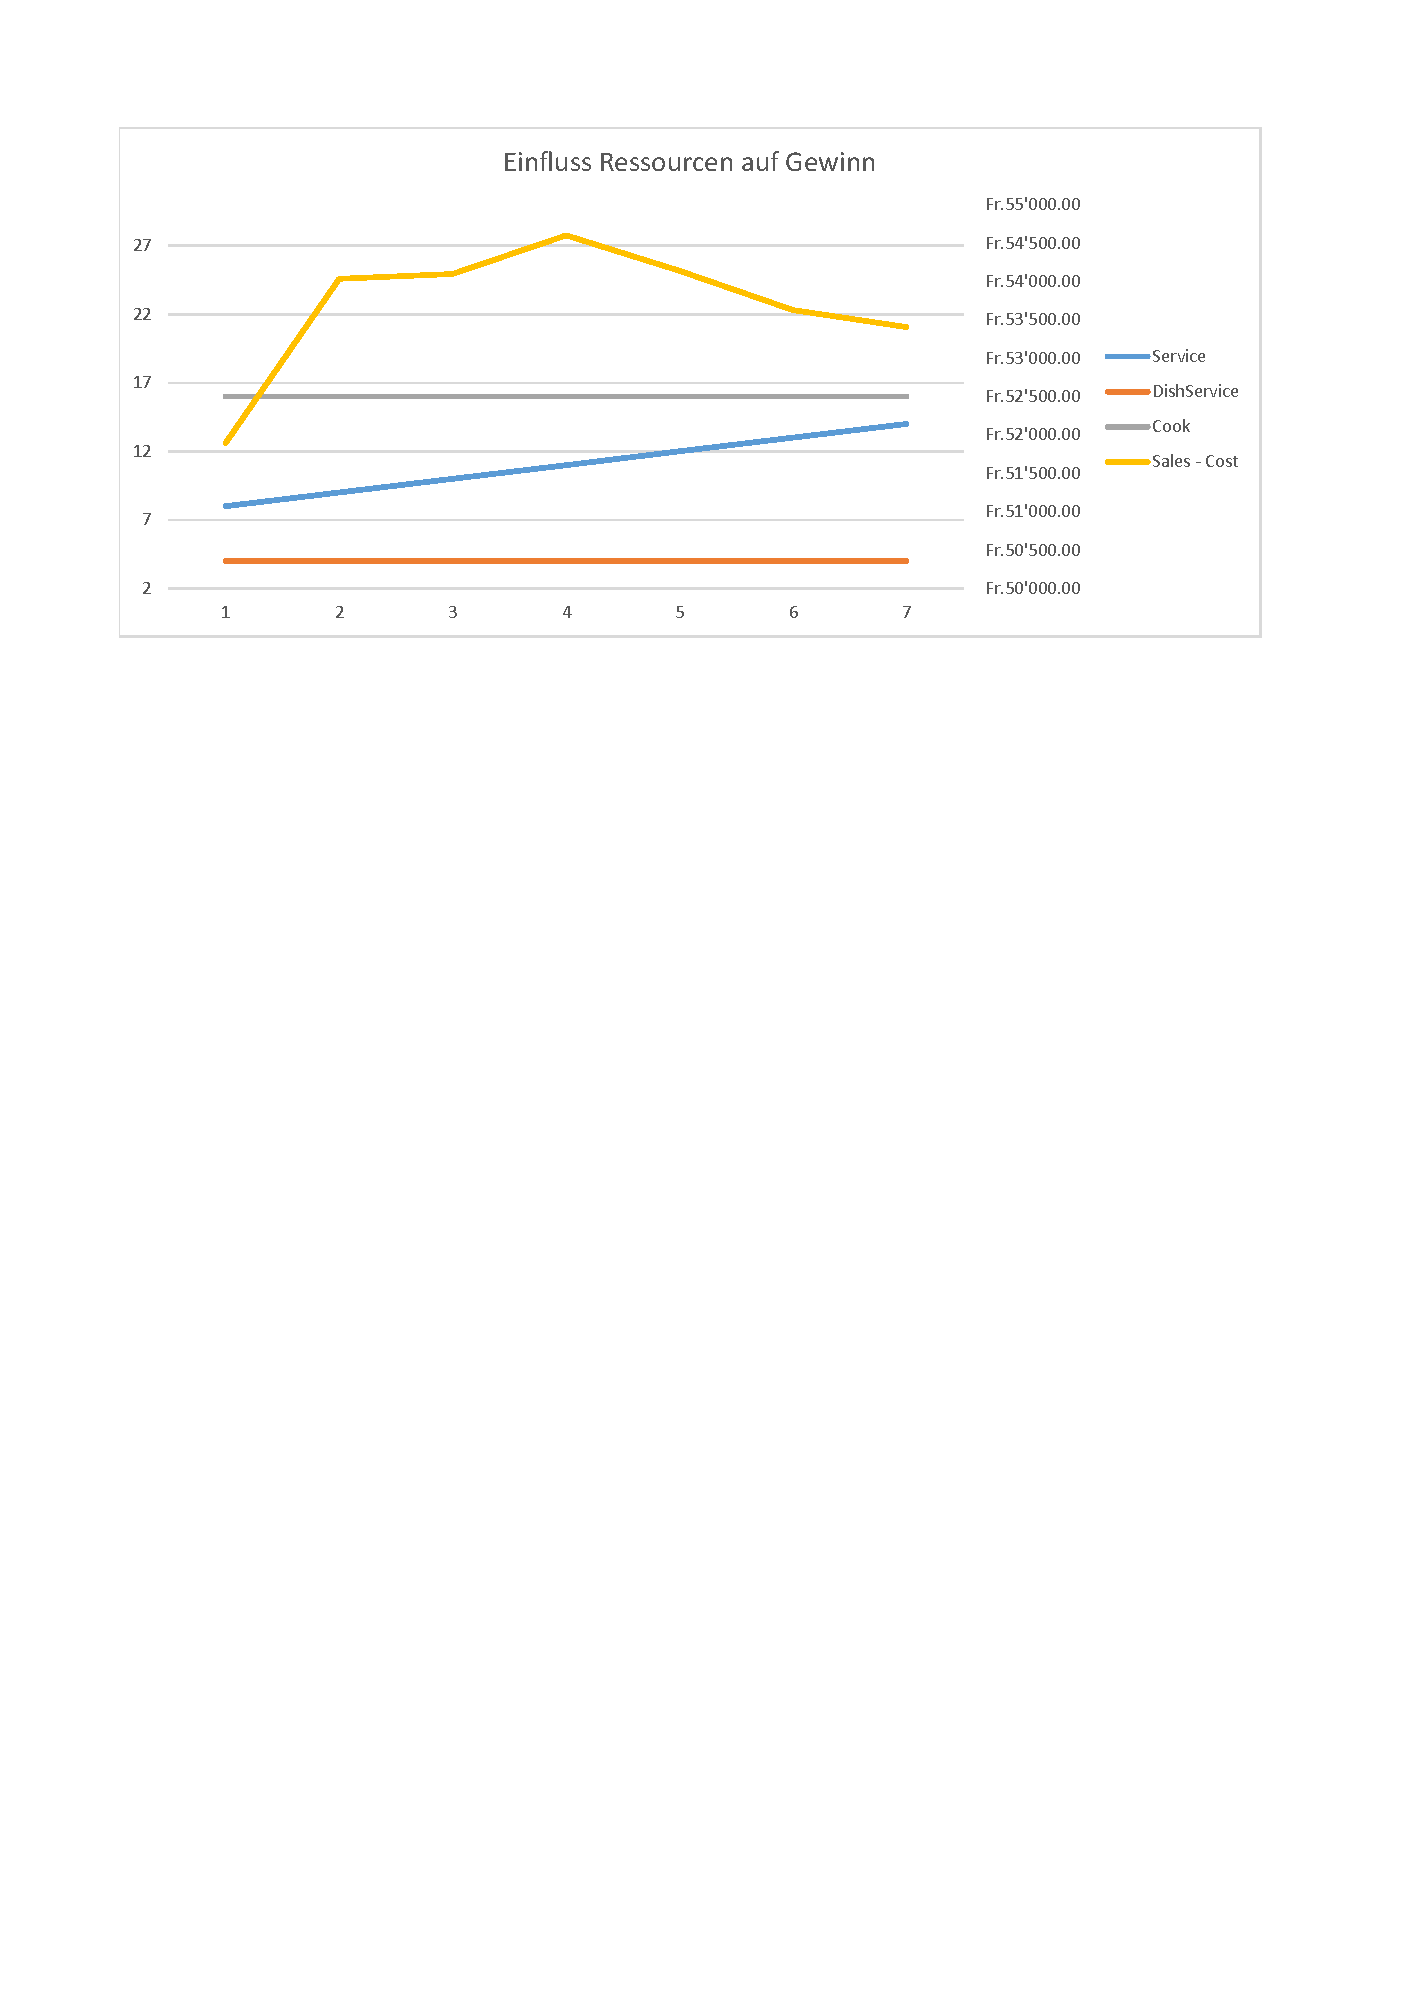
\includegraphics[trim=2cm 22.75cm 2.5cm 2cm, clip=true,width=\textwidth]{../Auswertung/2_Service.pdf}
						\caption[Serviceoptimierungsszenarien]{Serviceoptimierungsszenarien}
						\label{Serviceoptimierungsszenarien}
				\end{figure}
				
				Aus der erneuten Simulation geht hervor, dass sich die optimale Anzahl der Servicekräfte um 11 bewegt.
				
			\subsection{Tellerbringer}
				In einem weiteren Schritt fixieren wir das Servicepersonal bei 11 und die Köche bei 16 Personen, variieren aber die Tellerbringer zwischen 2 und 6.
				
				\begin{figure}[H]
					\centering
						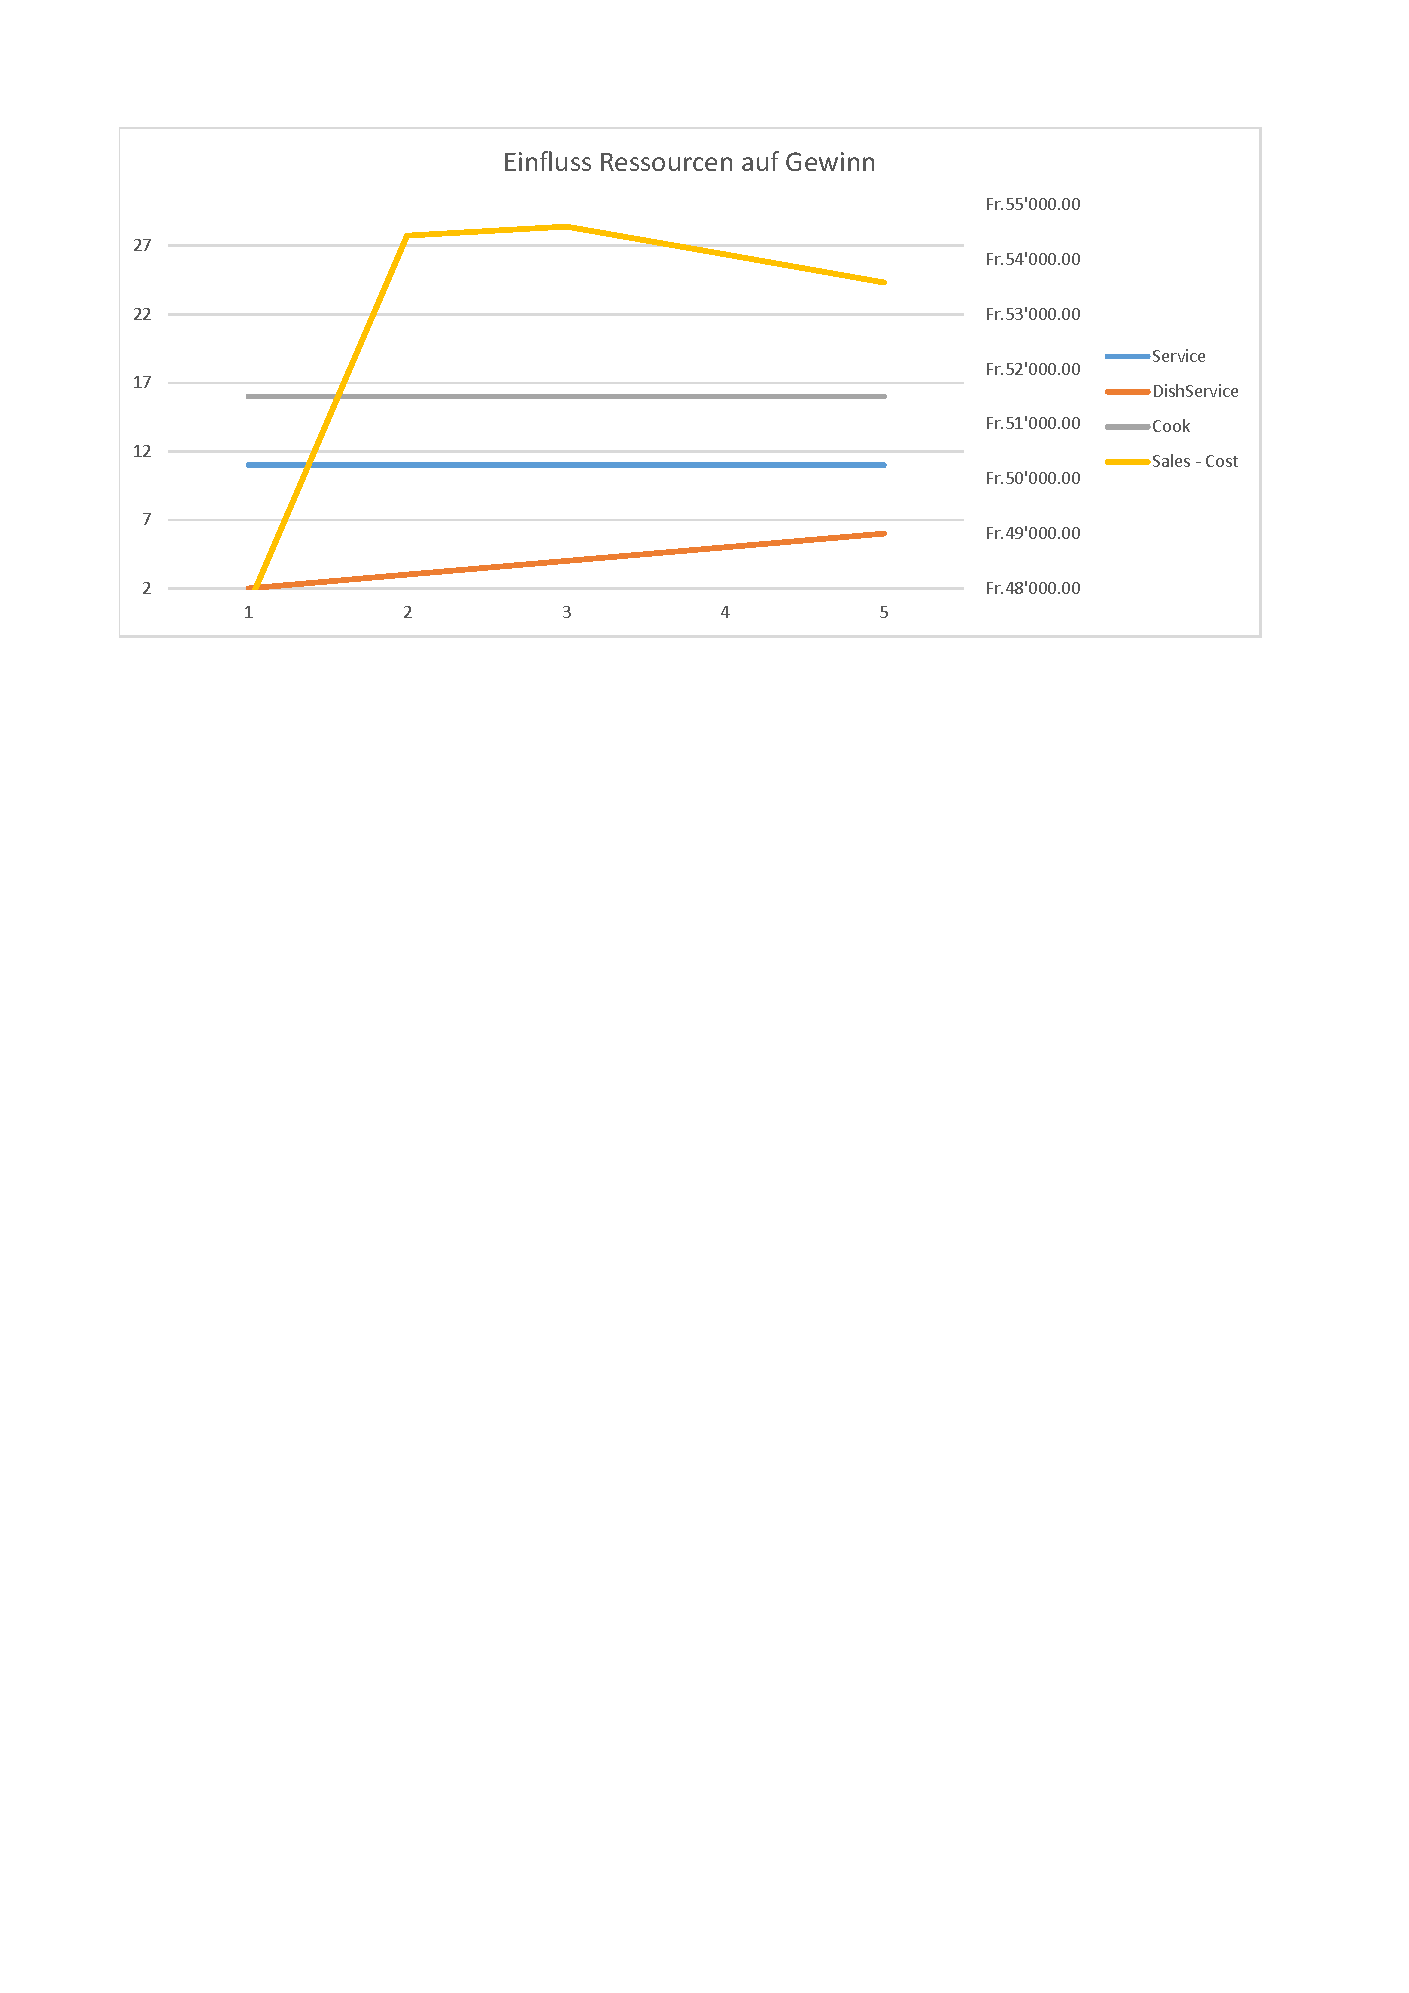
\includegraphics[trim=2cm 22.75cm 2.5cm 2cm, clip=true,width=\textwidth]{../Auswertung/3_DishService.pdf}
						\caption[Tellerbringeroptimierungsszenarien]{Tellerbringeroptimierungsszenarien}
						\label{Tellerbringeroptimierungsszenarien}
				\end{figure}				
				
				Aus den Ergebnissen der Simulationsläufe geht hervor, dass die optimale Anzahl Tellerbringer bei 3 liegt. Wir wählen für das weitere Vorgehen trotzdem eine Anzahl von 4, um auch mit einer grösseren Anzahl an Köchen die Menüs noch rauszubringen.

			\subsection{Köche}
				Im letzen Schritt fixieren wir die Tellerbringer und das Servicepersonal, variieren stattdessen die Köche zwischen 11 und 18 Personen.
				
				Die optimale Anzahl Köche liegt bei 14. Daraus ergibt sich ein Verhältnis von 11:4:14, bzw. 0.8 Servicekräfte auf 0.3 Tellerbringer auf einen Koch.

		
		\subsection{Dritte Selektion}
			Nach der Selektion muss überprüft werden, ob die einzelnen Optimierungen zu globalen Veränderungen geführt haben.
			
			Dazu erstellen wir 27 Szenarien, die das Servicepersonal zwischen 10 und 12, die Tellerbringer zwischen 3 und 5 sowie die Köche zwischen 13 und 15 variieren.
			
				\begin{figure}[H]
					\centering
						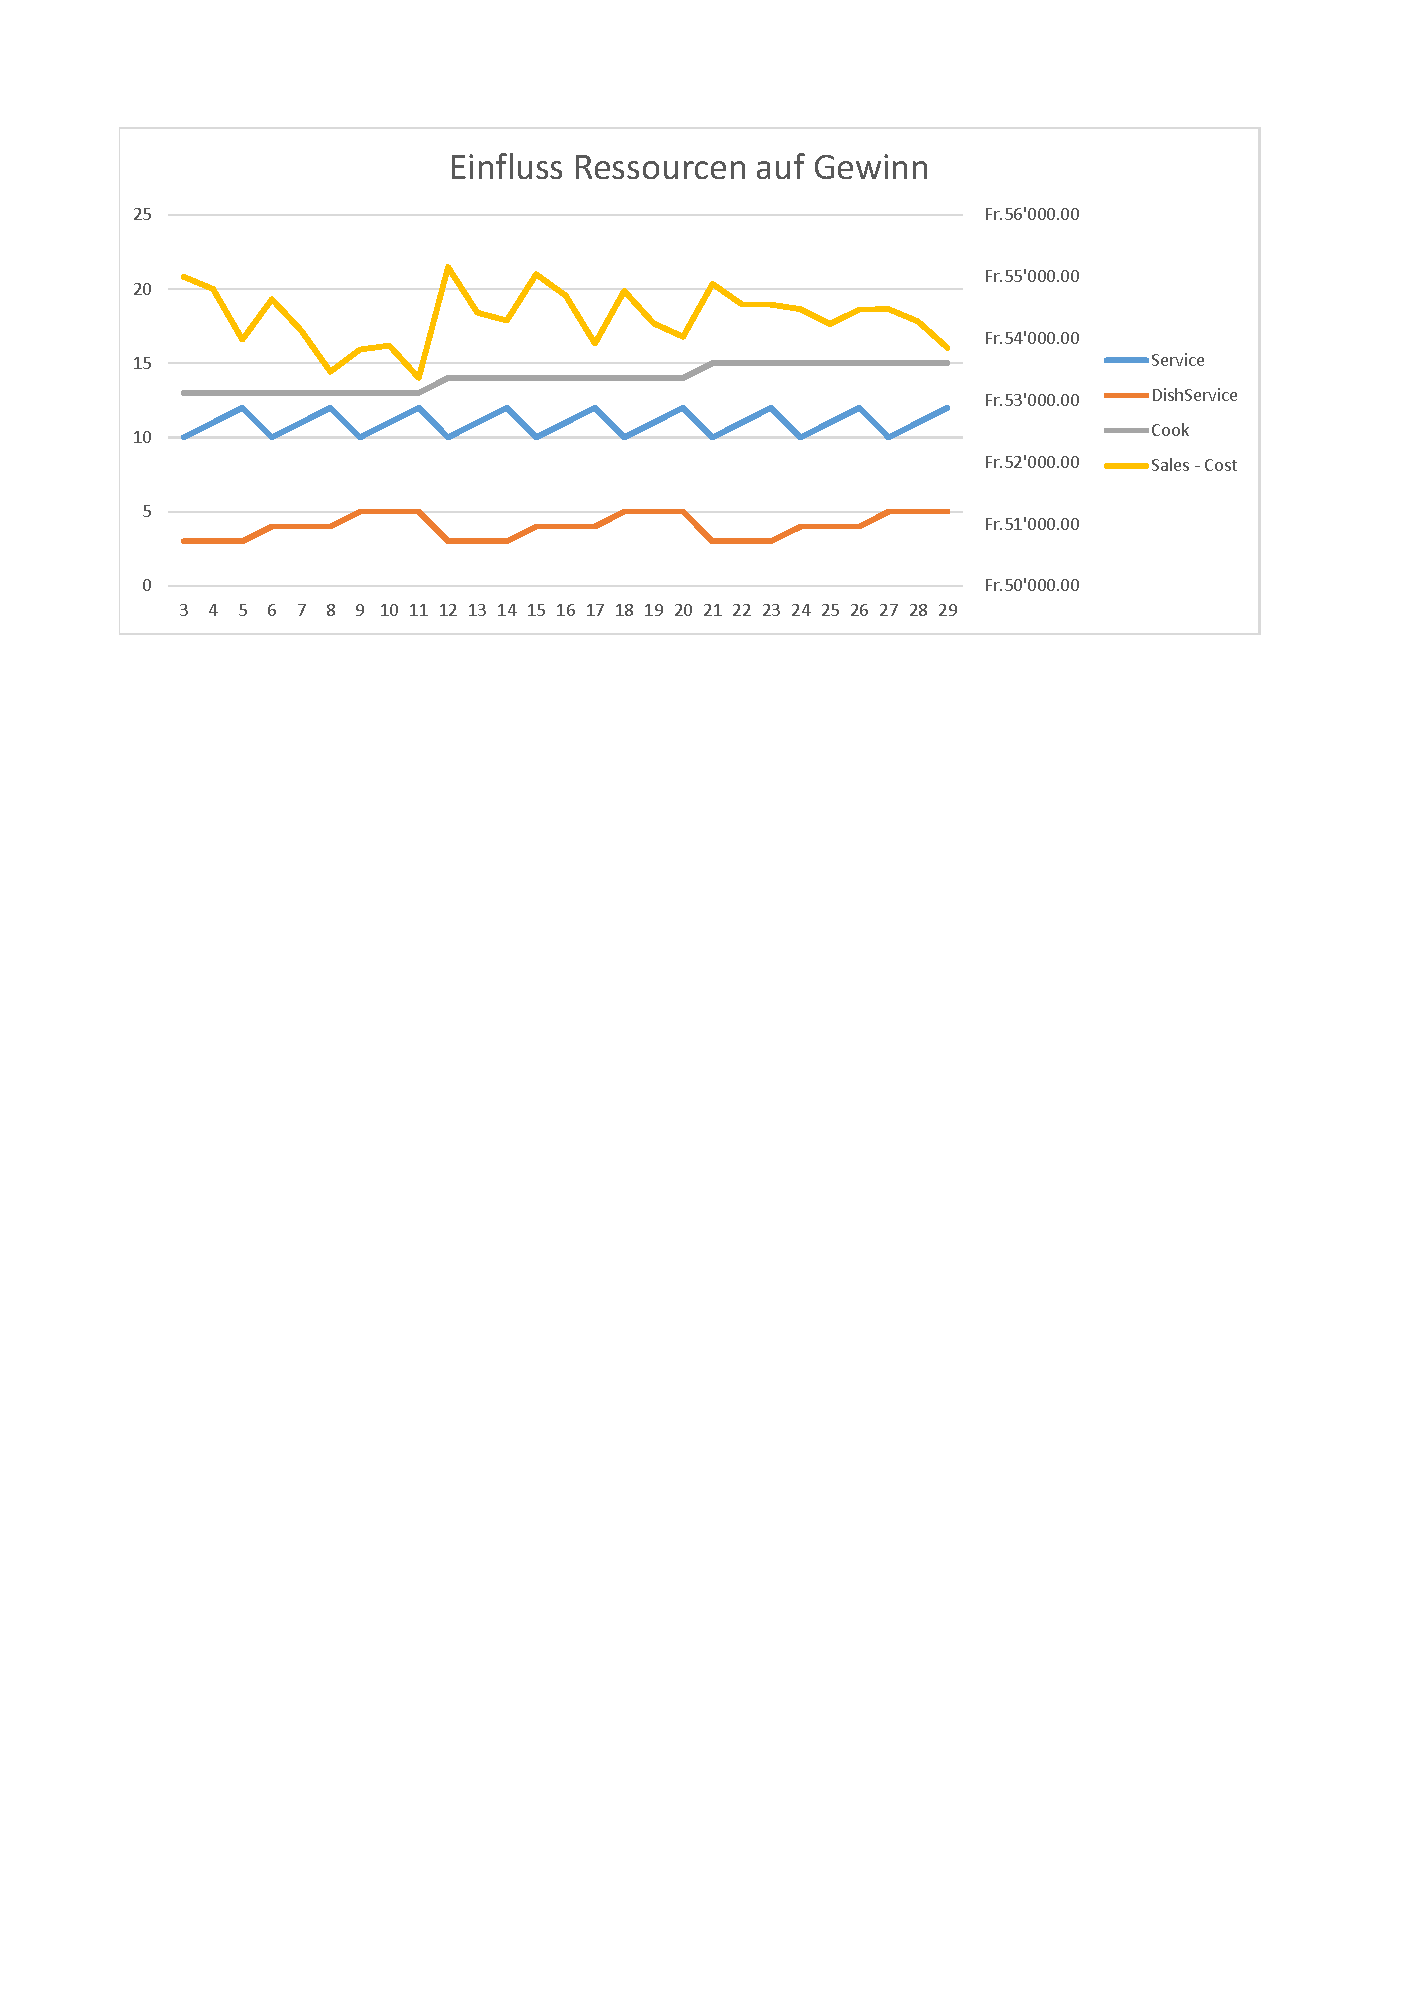
\includegraphics[trim=2cm 22.75cm 2.5cm 2cm, clip=true,width=\textwidth]{../Auswertung/4_+-1.pdf}
						\caption[Endoptimierung]{Endoptimierung}
						\label{Endoptimierung}
				\end{figure}	
			
			Die vier besten Resultate dieser Simulation erweisen sich als die allerbesten Resultate über alle bisherigen Szenarien hinaus. Alle diese Szenarien benötigen 10 Servicekräfte, die Tellerbringer variieren zwischen 3 und 4 und die Köche zwischen 13 und 15. Denr besten Fall erhalten wir mit 10 Servicekräften, 3 Tellerbringer und 14 Köchen.
			
			In einem nächsten Schritt müssten wir noch die Fälle auf zwei Tellerbringer und 9 oder 8 Servierkräfte ausdehnen, um sicher zu gehen, dass der optimale Fall gefunden wurde. Wir entscheiden uns jedoch für eine Verifikation mit den in Arena eingebauten Tools.
		
		\subsection{Verifikation}
			Zur Verifikation der Resultate nutzen wir OptQuest von Arena. Wir lassen OptQuest die Personalgrössen nach dem Gewinn optimieren. Arena liefert nach zwei Tagen Simulation beinahe das gleiche Resultat welches wir weiter oben erhalten haben. Lediglich für die Servicekräfte schlägt Arena eine Person weniger vor.
			\begin{figure}[H]
				\centering
					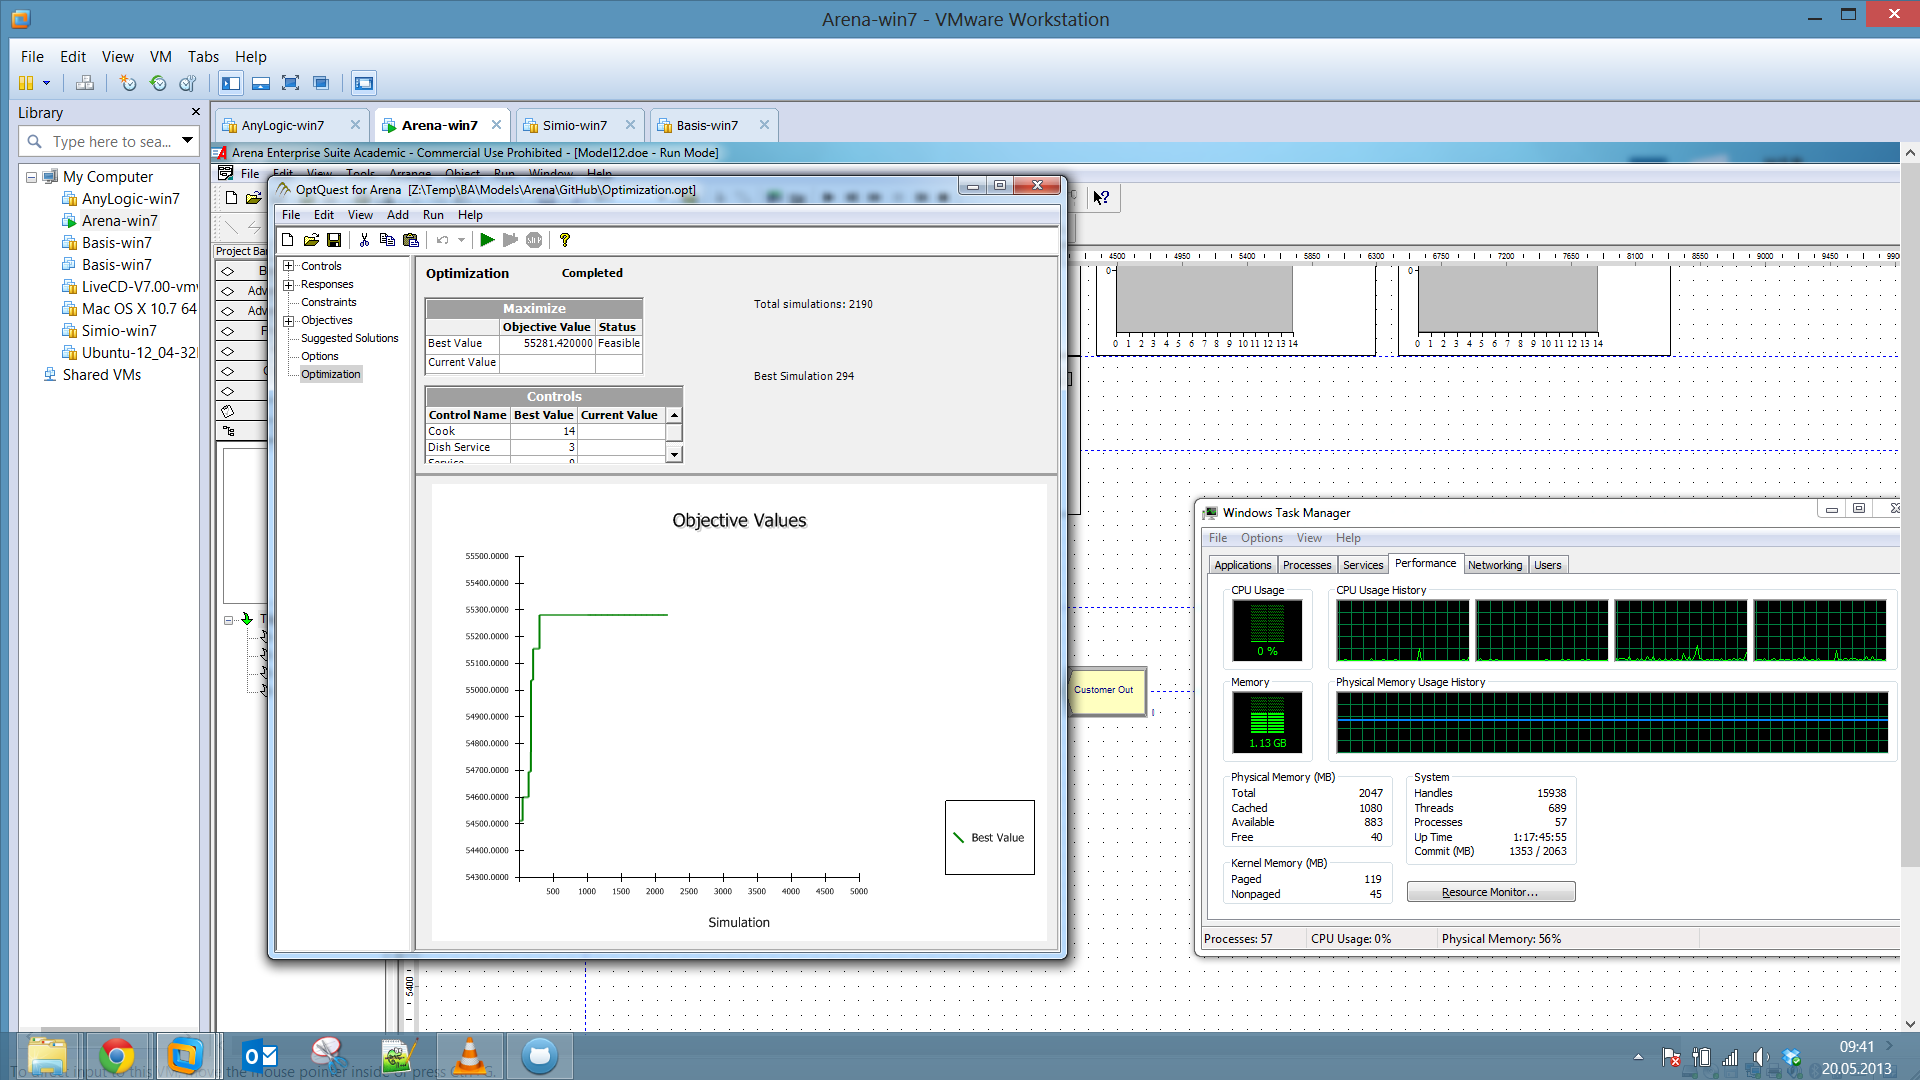
\includegraphics[width=\textwidth]{img/OptQuest.PNG}
					\caption[OptQuest in Arena]{OptQuest in Arena}
					\label{optQuestInArena}
			\end{figure}
			
			\begin{figure}[H]
				\centering
					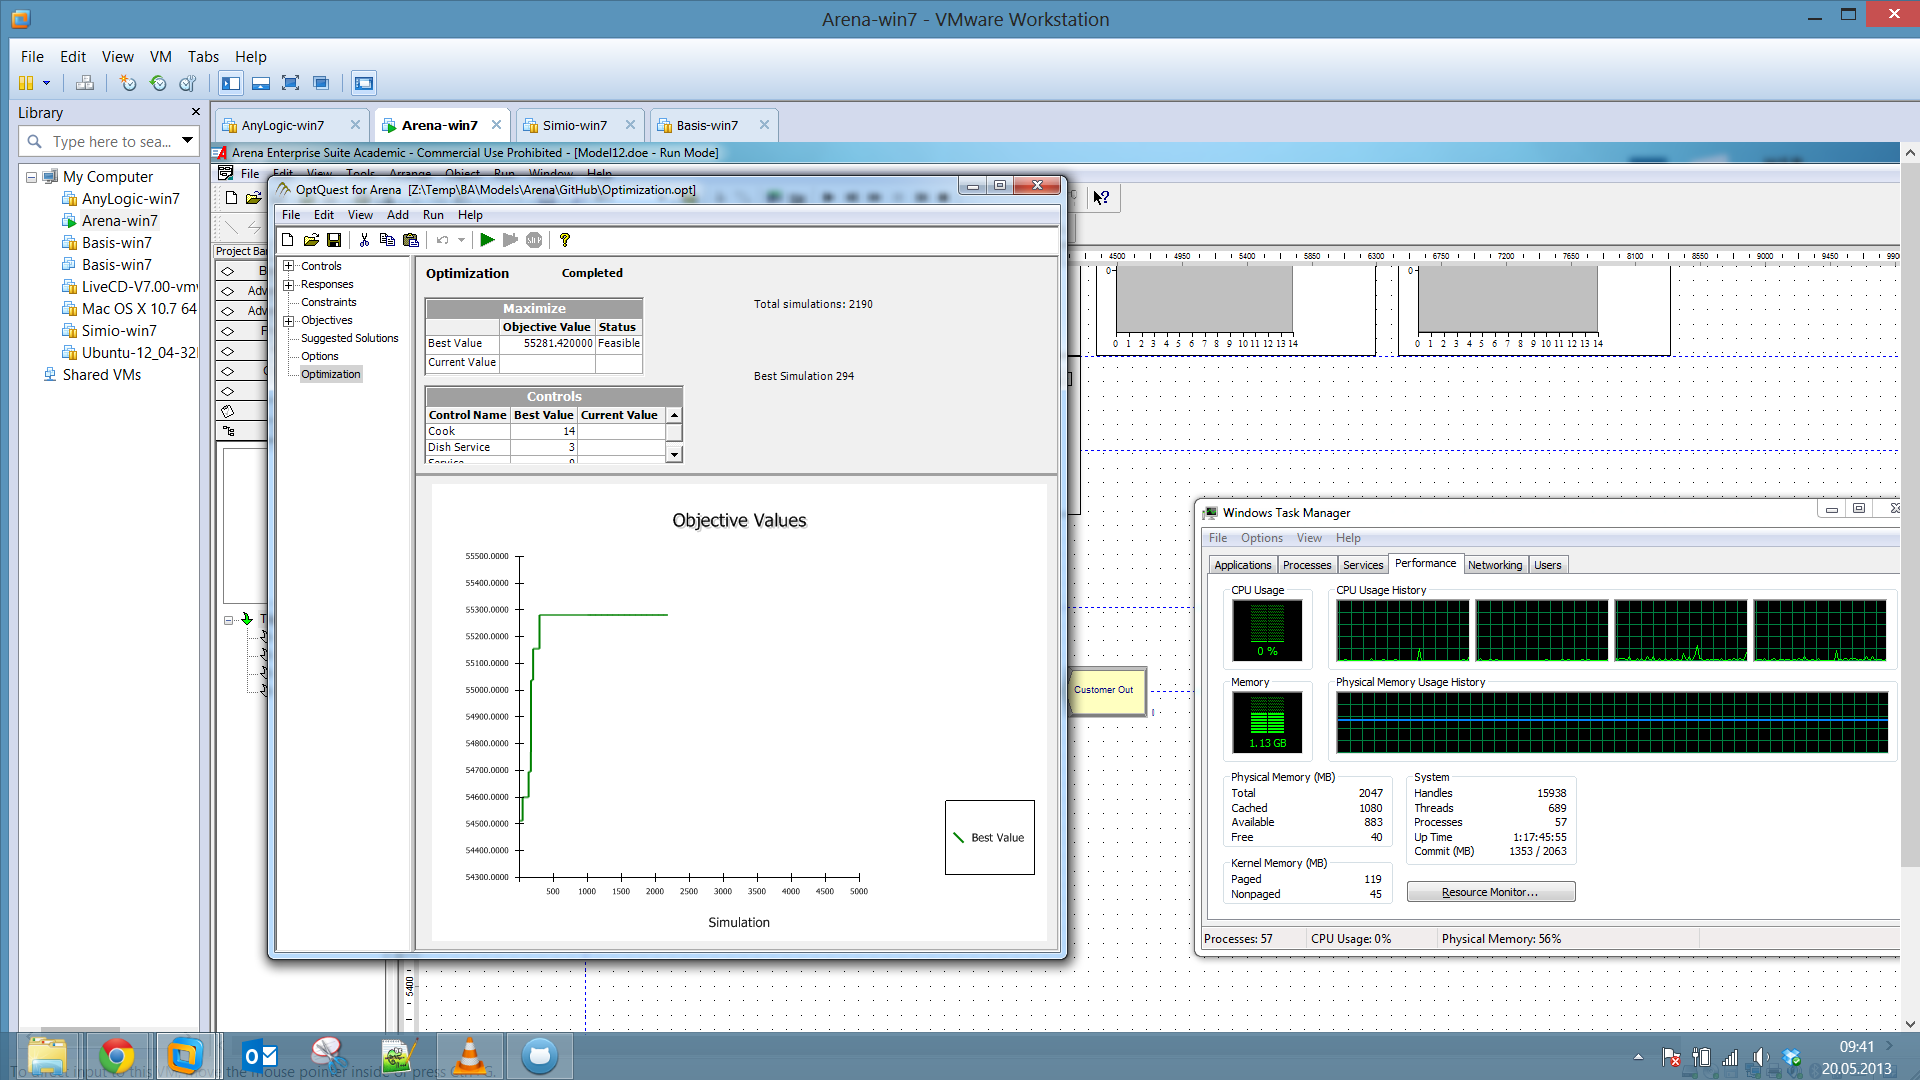
\includegraphics[trim=10cm 3.5cm 18.5cm 12.5cm, clip=true,width=0.75\textwidth]{img/OptQuest.PNG}
					\caption[OptQuest Suchverlauf]{OptQuest Suchverlauf}
					\label{optQuestSuchverlauf}
			\end{figure}
			
			Damit erhalten wir ein endgültiges Resultat von 14 Köchen, 9 Servierkräften und 3 Tellerbringer, die pro Tag über 55'200 CHF erwirtschaften (Umsatz - Löhne) und dabei über 1'700 Essen ausliefern. 
			
			Von diesem Betrag müssten natürlich noch sämtliche anfallende Kosten wie Nahrungsmitteleinkäufe, Infrastrukturkosten, Sozialabgaben und Personalausfälle abgezogen werden, wollte man mit den ermittelten Daten einen ernsthaften Businessplan aufstellen.

	\section{Fragestellungen (If Questions)}
		\begin{itemize}
			\item \textbf{Was passiert, wenn die Anzahl Köche erhöht wird?} \\
				Die Köche bringen eine grössere Menge an Bestellungen durch in der gleichen Zeit. Das Servicepersonal ist besser ausgelastet. Sobald das Verhältnis von Köchen zu Servicepersonal 1.4:1 übersteigt, sind die Servicerkräfte komplett ausgelastet, bzw. überlastet. Die Tellerbringer sind überlastet, sobald das Verhältnis von Köchen zu Tellerbringern 4.7:1 übersteigt.
			\item \textbf{Was passiert, wenn die Anzahl Köche verringert wird?} \\
				In der Küche stauen sich die Bestellungen. Die Gäste müssen zu lange auf das Essen warten. Zu wenige neue Gäste können in das Lokal eintreten, das Servicepersonal und die Tellerbringer sind ab den genannten Grenzen nicht mehr ausgelastet.
			\item \textbf{Was passiert, wenn die Anzahl Tellerbringer erhöht wird?}\\
				Sind zu viele Tellerbringer vorhanden, sind diese nicht ausgelastet und stehen herum.
				
			\item \textbf{Was passiert, wenn die Anzahl Tellerbringer verringert wird?}\\
				Sind weniger Tellerbringer als oben erwähnt vorhanden, stauen sich die gekochten Bestellungen in der Küche. Die Gäste erhalten wiederum die Bestellungen verspätet, belegen das Lokal länger und insgesammt sinkt die Anzahl Bestellungen, die durchgebracht werden können.
			\item \textbf{Was passiert, wenn die Anzahl Servicekräfte erhöht wird?}\\
				Werden die Servicekräfte erhöht, können mehr Bestellungen aufgenommen werden. Sobald das oben genannte Verhältnis zu den Köchen überstiegen wird, stauen sich die Bestellungen in der Küche und das Servicepersonal ist unterausgelastet.
			\item \textbf{Was passiert, wenn die Anzahl Servierkräfte verringert wird?}\\
				Die Servierkräfte können weniger Bestellungen aufnehmen. Die Küche und die Tellerbringer sind weniger stark ausgelastet.
			\item \textbf{Was passiert, wenn die Anzahl Plätze an der Bar verändert werden?}\\
				Wird die Platzzahl erhöht, so ist die Schlange vor der Türe kleiner und weniger Leute gehen wieder nach Hause. Das Restaurant ist länger besetzt und mehr Umsatz wird generiert. Ist die Bar zu gross, führt der Verzögerungseffekt dazu, dass Gäste noch nach Betriebsschluss im Lokal sind.
				
				Ist die Bar zu klein, gehen viele Leute wieder nach Hause, weil die Schlange vor der Tür zu lang ist. Weniger Gäste durchlaufen das Lokal und weniger Umsatz wird generiert.
			\item \textbf{Was passiert, wenn die Grösse der akzeptablen Schlange variiert wird, bis Gäste wieder nach Hause gehen?}\\
				Wird die Grösse angehoben, gehen weniger Leute nach Hause. Es braucht Mehr Personal im Lokal und die Gäste verbleiben durch den Verzögerungseffekt wie bei der Bar möglicherweise bis nach Betriebsschluss.
				
				Wir die Grösse verkleinert, so gehen mehr Leute nach Hause. Es wird weniger Personal benötigt und weniger Umsatz generiert.
		\end{itemize}


\appendix
\begin{landscape}
	\chapter{Simulationsdaten}
	\begin{center}
		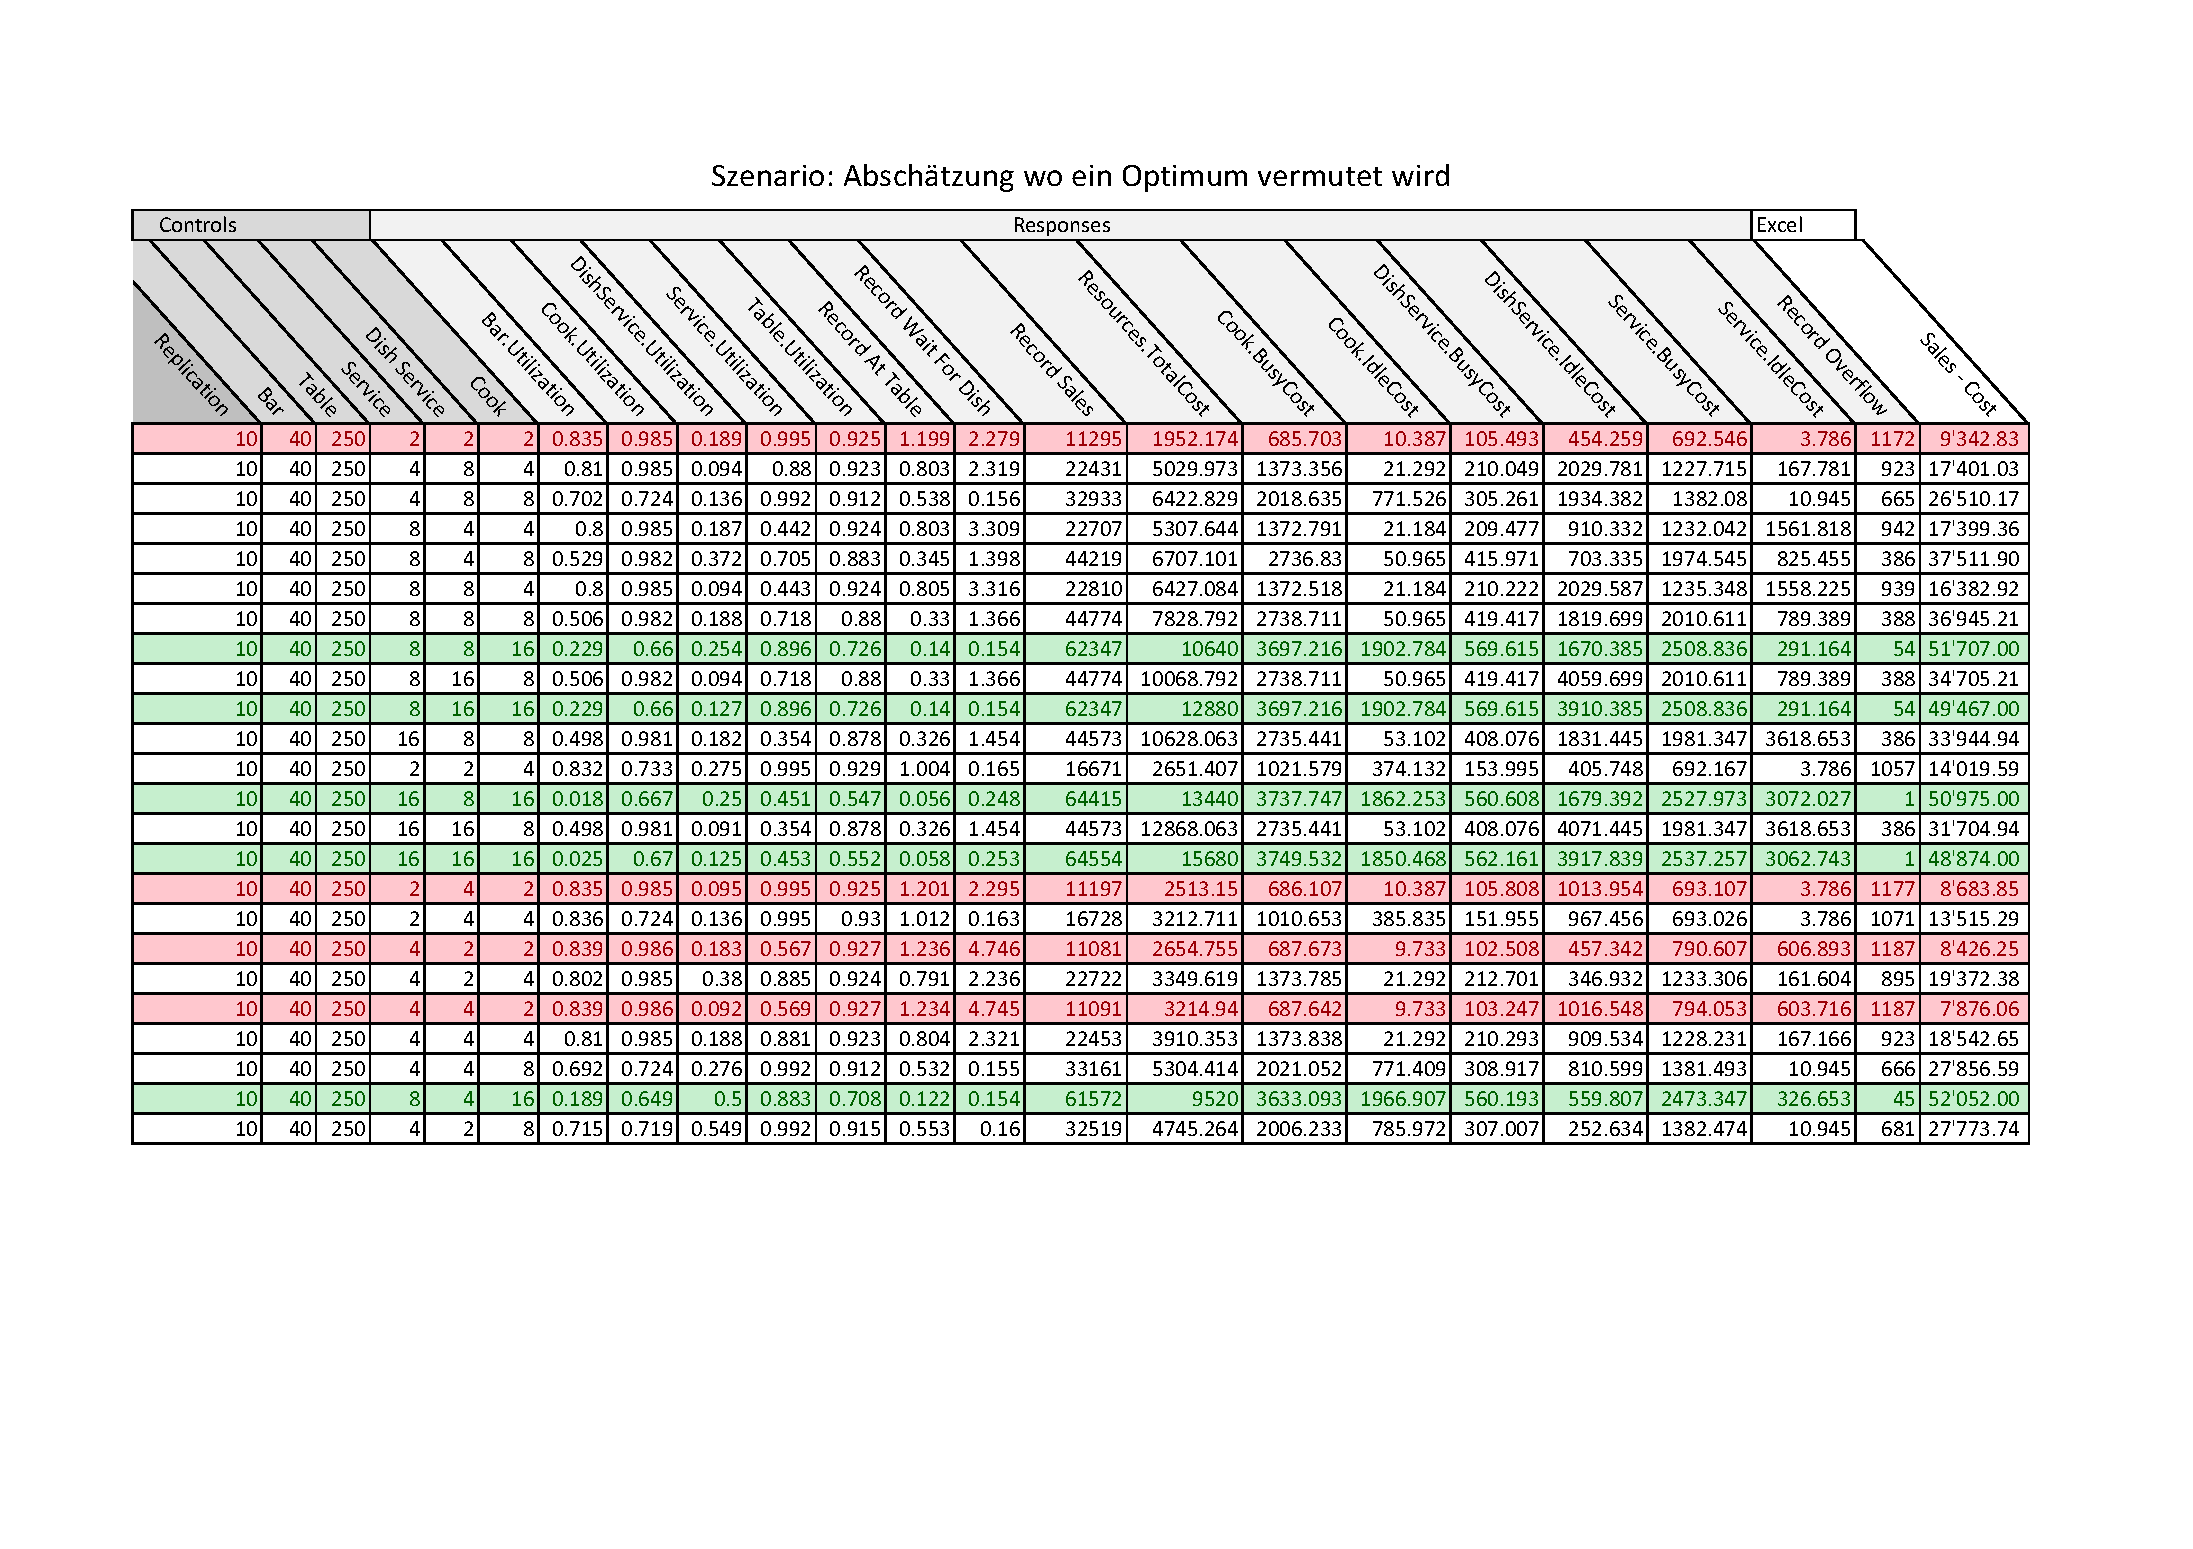
\includegraphics[page=1, trim=2cm 6cm 2cm 2cm, clip=true, width=1.35\textwidth]{../Auswertung/Data.pdf}
	\end{center}
	\begin{center}
		\includegraphics[page=2, trim=2cm 14cm 2cm 2cm, clip=true, width=1.425\textwidth]{../Auswertung/Data.pdf}
		\includegraphics[page=3, trim=2cm 15cm 2cm 2cm, clip=true, width=1.425\textwidth]{../Auswertung/Data.pdf}
	\end{center}
	\begin{center}
		\includegraphics[page=4, trim=2cm 5cm 2cm 2cm, clip=true, width=1.35\textwidth]{../Auswertung/Data.pdf}
	\end{center}
\end{landscape}


\chapter{Arena Report}
	\begin{figure}[H]
		\begin{center}
			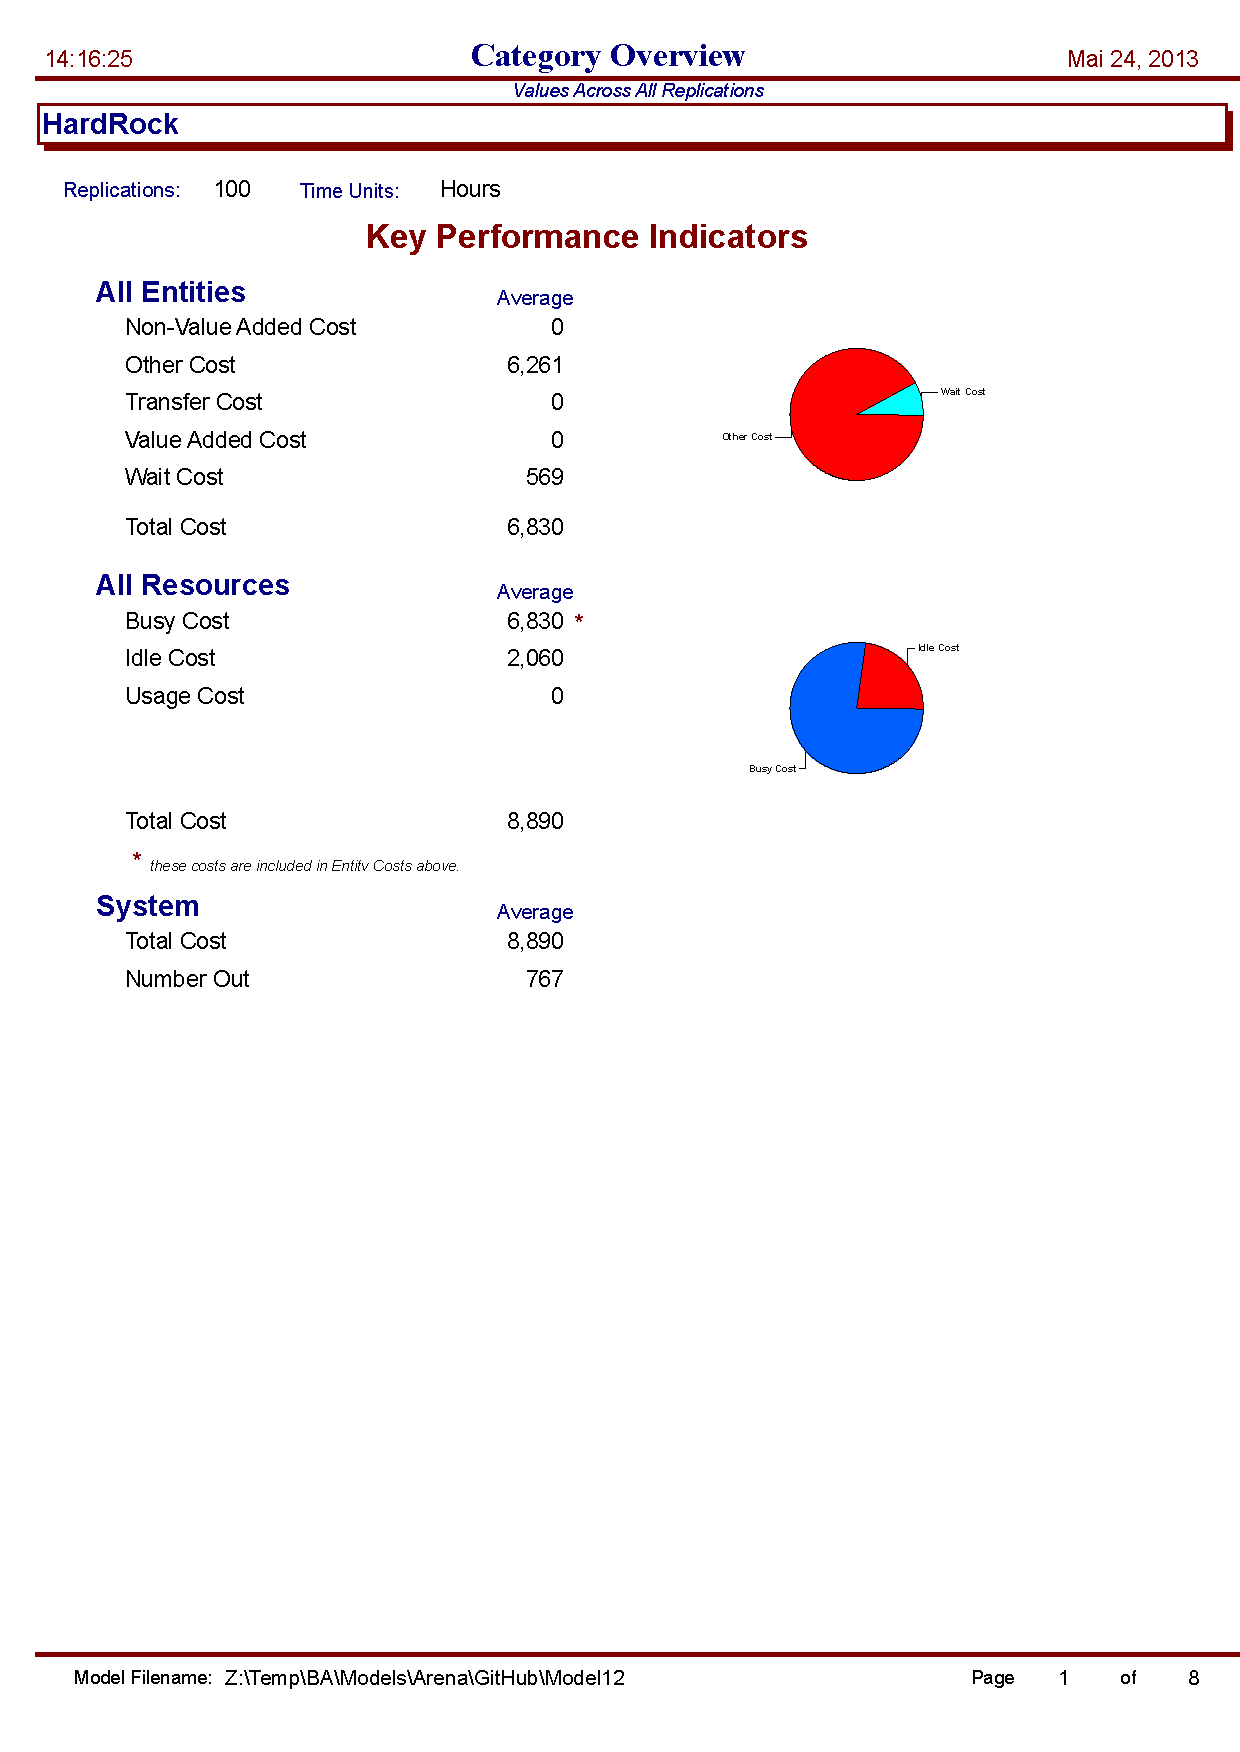
\includegraphics[page=1, trim=0cm 10cm 0cm 0cm, clip=true, width=\textwidth]{../Auswertung/Raport 14-3-9/category overview.pdf}
		\end{center}
	\end{figure}
	\begin{figure}[H]
		\begin{center}
		\includegraphics[page=2, width=0.95\textwidth]{../Auswertung/Raport 14-3-9/category overview.pdf}
		\end{center}
	\end{figure}
	\begin{figure}[H]
		\begin{center}
		\includegraphics[page=3, trim=0cm 0cm 0cm 0cm, clip=true, width=\textwidth]{../Auswertung/Raport 14-3-9/category overview.pdf}
		\end{center}
	\end{figure}
	\begin{figure}[H]
		\begin{center}
		\includegraphics[page=4, trim=0cm 0cm 0cm 0cm, clip=true, width=\textwidth]{../Auswertung/Raport 14-3-9/category overview.pdf}
		\end{center}
	\end{figure}
	\begin{figure}[H]
		\begin{center}
		\includegraphics[page=5, trim=0cm 0cm 0cm 0cm, clip=true, width=\textwidth]{../Auswertung/Raport 14-3-9/category overview.pdf}
		\end{center}
	\end{figure}
	\begin{figure}[H]
		\begin{center}
		\includegraphics[page=6, trim=0cm 0cm 0cm 0cm, clip=true, width=\textwidth]{../Auswertung/Raport 14-3-9/category overview.pdf}
		\end{center}
	\end{figure}
	\begin{figure}[H]
		\begin{center}
		\includegraphics[page=7, trim=0cm 0cm 0cm 0cm, clip=true, width=\textwidth]{../Auswertung/Raport 14-3-9/category overview.pdf}
		\end{center}
	\end{figure}
	\begin{figure}[H]
		\begin{center}
		\includegraphics[page=8, trim=0cm 0cm 0cm 0cm, clip=true, width=\textwidth]{../Auswertung/Raport 14-3-9/category overview.pdf}
		\end{center}
	\end{figure}
	

\chapter{Präsentation Projektvorstellung}
\begin{center}
	\includegraphics[page=1,angle=180, scale=0.67]{media/presentation-hardrock-slides.pdf}
\end{center}
\begin{center}
	\includegraphics[page=2,angle=180, scale=0.8]{media/presentation-hardrock-slides.pdf}
\end{center}
\begin{center}
	\includegraphics[page=3,angle=180, scale=0.8]{media/presentation-hardrock-slides.pdf}
\end{center}
%\includepdf[pages=1-3,angle=180, scale=0.9]{media/presentation-hardrock-slides.pdf}

\listoffigures

\begin{landscape}
%\chapter{Projekt Log}
%git log --no-merges --pretty=format:'%ci: %d %s <%an>' > documentation/gitLog.txt
%\verbatiminput{gitLog.txt}
\end{landscape}

\chapter{Materialnachweise}
\section{Titelblatt}
\begin{tabularx}{\textwidth}{|Xlr|}
		\hline
		Logo Hardrock & www.hardrock.com & 25.03.2013 \\
		\hline
\end{tabularx}

\end{document}
